% COPY AND PASTE THE CODE THROUGH "START YOUR DOCUMENT" FOR EACH NEW REPORT
% - - - - - - - - - - - - - - - - - - - - - - - - - - - - - - - - - - - - - - - - - -
\documentclass[12pt]{article}

% import mathy things
\usepackage{amssymb}
\usepackage{amsmath}
\usepackage{amsthm}
\usepackage{booktabs}
\usepackage{float}
\usepackage[export]{adjustbox}
\newtheoremstyle{exmp}{3pt}{3pt}{\small}{\parindent}{\bfseries}{:}{0.5em}{}
\theoremstyle{exmp}
\newtheorem{example}{Example}

% use pictures and colors
\usepackage{graphicx}
\usepackage[usenames,dvipsnames]{color}
\usepackage{xcolor}

\usepackage[font=footnotesize]{caption}

% set page margins
\usepackage[top=1in, bottom = 0.7in, left=1in, right = 1in,letterpaper]{geometry}

\usepackage{hyperref}
\usepackage{enumerate}
% usepackage{epstopdf} 	%% uncomment to import .eps files on a Mac.
\usepackage{mdwlist}
\usepackage{ulem}
\usepackage{fancyhdr}
\usepackage{lastpage}

%\linespread{1.1}	% slightly more than single-spaced lines

% = = = = = = = = [BEGIN DO_NOT_EDIT]= = = = = = = = = = = = = =
%% Define custom commands for scientific review
%\newcommand\reporttitle[1]{{#1}}
%\newcommand{\reportsubtitle}[1]{{\large Application Excursion \#{#1}}\\[-0.5em]{\normalsize\textsc{Math 295: Computational Modeling}}}
%% setup for title and author(s)
%\makeatletter
%\newcommand{\makeReportTitle}{% 
%\title{\reporttitle \\ \reportsubtitle{\reportnumber}}
%
%  \@ifundefined{authortwo}{%
% 	\author{\authorone}%
%	}{%
%	\@ifundefined{authorthree}{%
%  		\author{\authorone \and \authortwo}%
%		}{%
% 		\author{\authorone \and \authortwo \and \authorthree}%
%		}}%
% 
%\maketitle
%\thispagestyle{empty}
%}
%\makeatother

% customize page numbers -- typeset TWICE to update page reference (eliminates ??)
\pagestyle{empty}
\makeatletter \renewcommand{\@evenhead}{%
%\normalsize\slshape DRAFT \today\hfil \upshape %
\small \texttt{Team \#~1926166 \hfill  {Page~\thepage} of \pageref{LastPage}}} \renewcommand{\@oddhead}{\@evenhead} \makeatother

% - - - - - - - - - - - - - - - - - - - - - - - - - - - - - - - - - - 
% = = = = = = = = [END DO_NOT_EDIT]= = = = = = = = = = = = = = 


















% = = = = = = = = = = = = = = = = = = = = = = = = = = = = = = 
%		SETUP TITLE PAGE -- UPDATE {content} FOR EACH NEW ASSIGNMENT
% = = = = = = = = = = = = = = = = = = = = = = = = = = = = = = 

% DEFINE A DESCRIPTIVE REPORT TITLE GIVEN THE TOPIC OF YOUR REPORT
\title{}
%\author{Team 93321}% per ICM instructions, DO NOT include your names!
\date{}

% = = = = = = = = = [END TITLE PAGE SETUP] = = = = = = = = = = = = 				
% = = = = = = = = = = = = = = = = = = = = = = = = = = = = = = 








% = = = = = = = = = = = = = = = = = = = = = = = = = = = = = = 
%				START YOUR DOCUMENT
% = = = = = = = = = = = = = = = = = = = = = = = = = = = = = = 
\begin{document}		% Text will appear after this command


% make title page - DO NOT EDIT
\makeatletter
%\maketitle
\thispagestyle{fancy} 
\chead{\small \texttt{Team \#~1926166 \hfill  {Page~\thepage} of \pageref{LastPage}}} 
\makeatother
% = = = = = = = = = = = = = = = = = = = = = = = = = = = = = = 

% - - - - - - - - - - - TABLE OF CONTENTS - - - - - - - - - -
\tableofcontents 	% Typeset 2 or 3 times to update page numbers in table of contents

% - - - - - - - - - - - REPORT STARTS HERE - - - - - - - - - -


% - - - - - - - - - - - Introduction - - - - - - - - -
\newpage
\section{Introduction} 
\label{sec:introduction} 
\subsection{Problem Background}
In recent years, the United States is facing a countrywide problem with respect to drug abuse as prescription use and  illicit recreational use. Drug abuse will undermine human health and personal property as using drugs disorderly may cause hepatitis, HIV infection, and also neonatal abstinence syndrome. Federal government and organizations are trying their best to ``save lives and prevent negative health effects of this epidemic''.[1] Thus, for the purpose of countering the opioid crisis, in this paper we will: \begin{itemize}
    \item Use the 2010-2017 NFLIS data provided to model the spread and find the characteristics of the reported synthetic opioids and heroin incidents in and between the five states, Ohio, Kentucky, West Virginia, Virginia, and Pennsylvania in terms of their counties for trend analysis.
    \item Use the U.S Census socio-economic data provided to improve the model we constructed and give a more precise % need to be modified
    \item Identify strategies for countering the opioids crisis.
\end{itemize}


\subsection{Previous Research}
Since this topic involves the interaction between adjacent counties, it is very similar to the model focusing on infectious disease propagation. We looked up for various researches about this topic and found that most of them are based on Cellular Automaton algorithm (CA), such as Yu Lei, Xue Hui-Feng, Gao Xiao-Yan, and Li Gang's research on the transmission of SARS in 2007.[2] Mushayabasa's work on illict drug use dynamics is also very related to our topic.[3] The major work that we refer to is Sirakoulis, Karafyllidis, and Thanailakis's research about effects of population on epidemic propogation.[4] %Other works like Steady Mushayabasa's research on illicit drug use in South Africa use his own mathematical model to illustrate the numerical results in 2015.%NEED MORE WORK ON THIS
%The major work that we refer to is the Steady Mushayabasa's research paper and his model.

\subsection{Our work}
In this solution, we first, by referring to Sirakoulis et al's model, build the CA model for the spread of drugs that we can apply data of heroine or synthetic opioid from the year 2010 to 2017 with the provided NFLIS data, analyze patterns and characteristics of the reports, and evaluate the future trends as well as origin locations based upon the model. Then we add the U.S. Census socio-economic data into consideration, by which we find influential factors from the data set that help explain the drug-use trend. For the last part, we would modify the influential factors in the model to determine a possible strategy for countering the opioid crisis.

 % labels allow you to cross-reference a section later in the document, without having to remember its number
%  - - - - - - - - - - - - - - - - - - - - - - - - - - - - - -
% Delete existing text when writing your own report.


 

% - - - - - - - - - - - END Introduction - - - - - - - - - - -


% - - - - - - - - - - - Model Design - - - - - - - - -
\section{Assumptions} 

\begin{itemize}
    \item The NFLIS data and US Socio-economic data are correct as provided.
    
    \item Drug can only be transported from one county to its adjacent counties. 
    
    \item The number of people who stop taking drugs forever after drug treatment is neglected.
    \item The population in each county will remain constant over years. 
    \item People only acquire drugs in the county that they are residing.
    \item In every year, the county which has nonzero drug reports will influence its adjacent counties merely by increasing each one's number of drug reports.
    %\item In every year, the number of drug reports in a county will decrease merely because of law enforcement.
    %Since the rate of drug relapse is relatively high (about 85$\%$) within a year after drug treatment action, we assume that once one got addicted to drugs, he or she will constantly be dependent on drugs.[4]
    % remember to reference the 85% data.
    % delete the third one. Conjecture: Since only 85% of addicted people can withdraw, drug reports in each county will keep increasing unless a law enforcement
    
\end{itemize}

%---------------------End Assumption------------------------

\vspace{-.5em}
\begin{table}
\centering
\begin{tabular}{c|l}
\toprule \\
Nomenclature & Meaning \\
\hline
$t$ & time with unit of year\\

$(i,j)$ & spatial coordinates for each cell, i.e. county\\

$C_{i,j}^t$ & the state of the ($i,j$) CA cell during year $t$\\

$S_{i,j}^t$ & the number of reports for the certain opioid in $(i,j)$ cell during year $t$.\\

INF$_{i,j}^t$ & "infectious flag" with only binary values 0 and 1\\

$\kappa$ & threshold value for the annual number of opioid reports within a county.\\

$\rho$ & the self increasing rate of a county if the number of reports in that county $>\kappa$\\

$k$ & the coefficient that represents the effect of the neighbors sharing a side with the cell\\

$l$ & the coefficient that represents the effect of the diagonal neighbors of the cell.\\

$r_t$ & the number of reports in the year of $t$
\bottomrule
\end{tabular}
\end{table}
% labels allow you to cross-reference a section later in the document, without having to remember its number
%  - - - - - - - - - - - - - - - - - - - - - - - - - - - - - -
% Delete existing text when writing your own report.

\section{Spread and Characteristics of Synthetic Opioids and Herion Incidents}

In this section, we are going to build a CA model to describe and predict the trends of the drug usage in the five states we are focusing on: Ohio, Kentucky, West Virginia, Virginia, and Pennsylvania. First we categorize the list of narcotic analgesic by synthetic, semi-synthetic, and non-synthetic opioids. Then the list of synthetic opioids contains all drugs other than Buprenorphine, Codeine, Heroin, Hydrocodone, Hydromorphone, Hydorcodeinone, Morphine, Opiate, Opium, Oxycodone, Oxymorphone, and Thebaine.

For heroin and synthetic opioids, we make heat maps for the number of drug reports within the five states from 2010 to 2017 respectively.  Using these graphs, we can easily visualize the trends of drug usage and trace its development along the timeline. Then, referring to Sirakoulis et al's work, we construct the corresponding CA model, which can be successfully tested by the given data in eight years. By using this model, we are able to predict the future trend-in-use and, in a reversed direction, locate the starting points of specific opioids in each of five states.  

 
\subsection{Geographical Visualization of Drug Reports}
In the following graphs, we use different shades of blue colors and orange colors to represent the number of heroin and synthetic opioid reports from the year of 2014 to 2017. The blue colors represent the number of annual Heroin reports in each county and the orange colors represent that of synthetic opioids.  The deeper the color of the county is, the more reports that county had in that year.
Since the numbers of annual reports about Herion increase at roughly the same rate as year passes during 2010-2013, we only show the distribution of annual reports geographically during 2014-2017, where significant and noteworthy changes occurred. The situation is similar to that of synthetic opioids, so we would also do the same thing to them.

 As told by the data, the number of annual Heroine reports experienced a mild growth every year. On the other hand, the amount of synthetic opioids reports  experienced a dramatically growth from year 2014 to year 2017, especially in Ohio.  As a result, the pictures we showed are chosen specifically for these changes.

%----------------------------------------------------------------
%----------------------ADD IT BACK!!!----------------------------
%----------------------------------------------------------------

\begin{figure}[H]
  \begin{minipage}{0.48\textwidth}
     \centering
     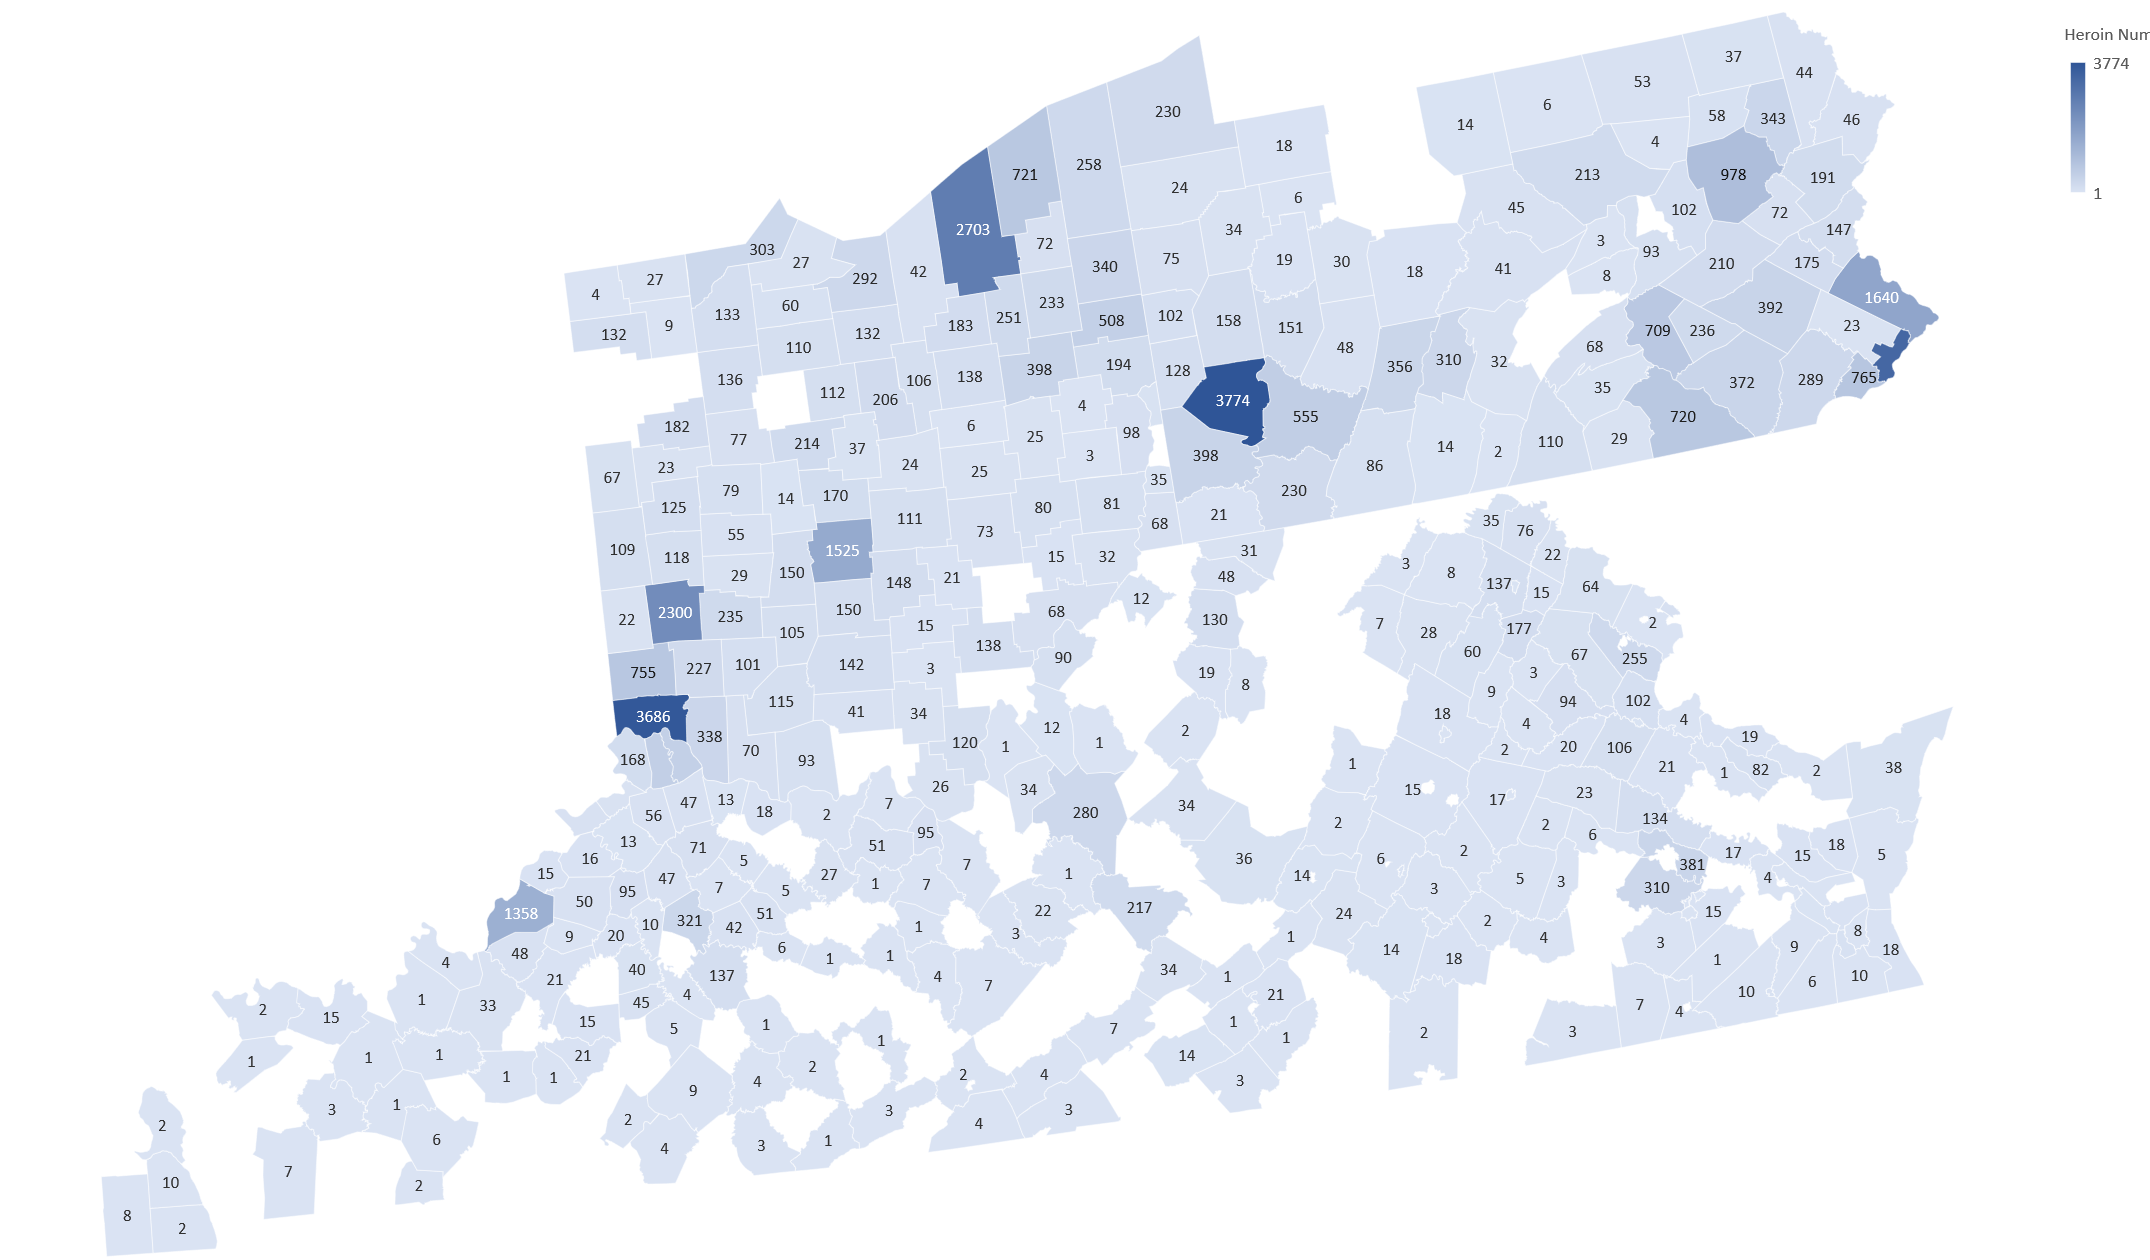
\includegraphics[width=\linewidth]{2014.png}
     \caption{Heroin Reports in 5 states in 2014}\label{H14}
  \end{minipage}%\hfill
  \begin{minipage}{0.48\textwidth}
     \centering
     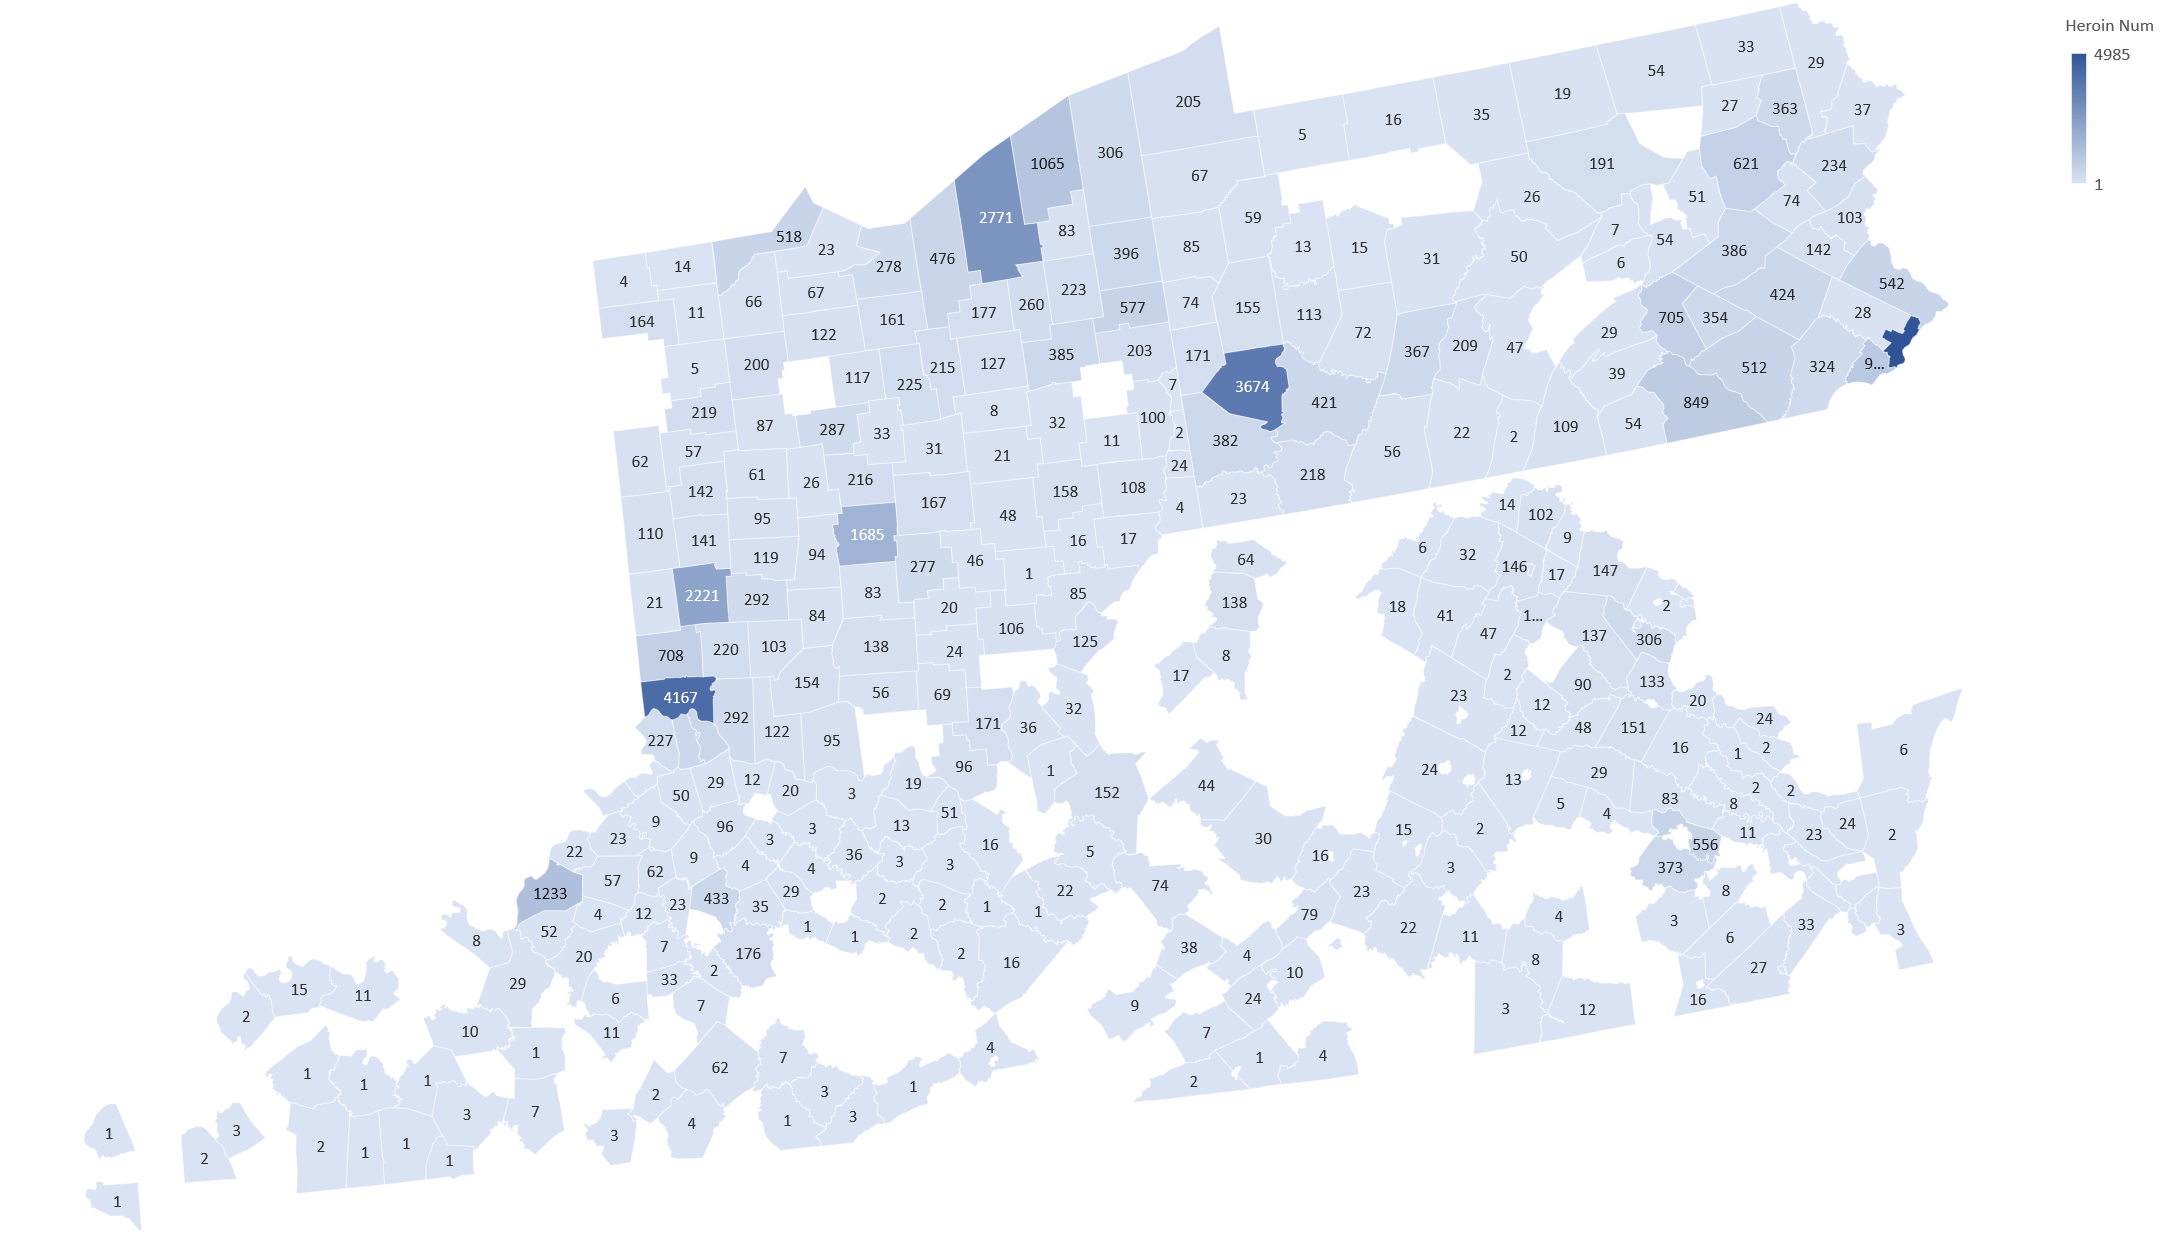
\includegraphics[width=\linewidth]{2015.png}
     \caption{Heroin Reports in 5 states in 2015}\label{H15}
  \end{minipage}
\end{figure}

\begin{figure}[H]
  \begin{minipage}{0.5\textwidth}
     \centering
     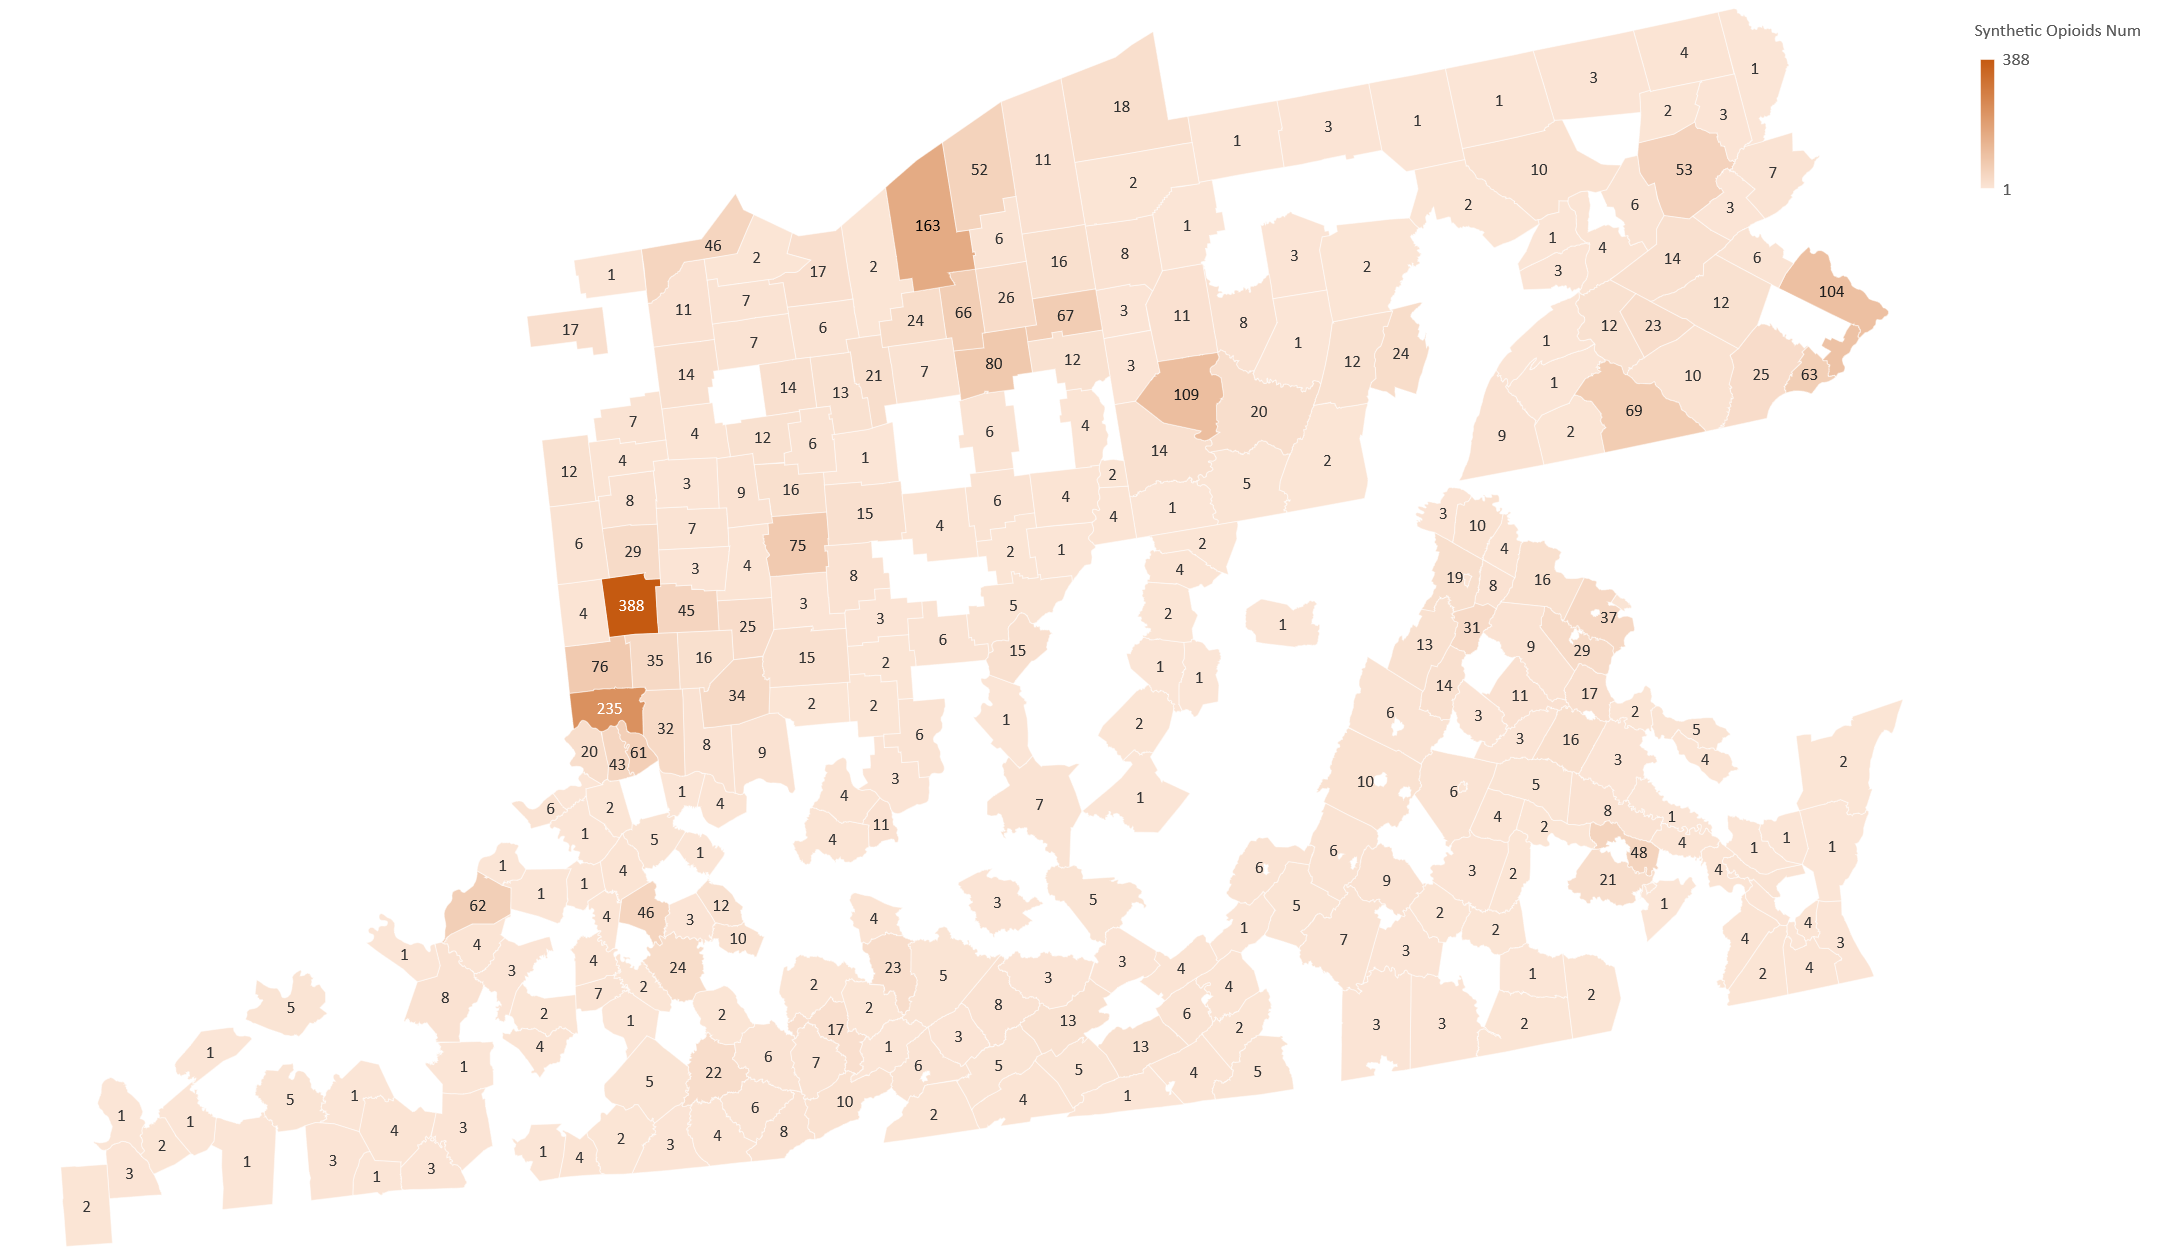
\includegraphics[width=\linewidth]{2014SYN.png}
     \caption{Synthetic Opioids Reports in 5 states in 2014}\label{S14}
  \end{minipage}%\hfill
  \begin{minipage}{0.5\textwidth}
     \centering
     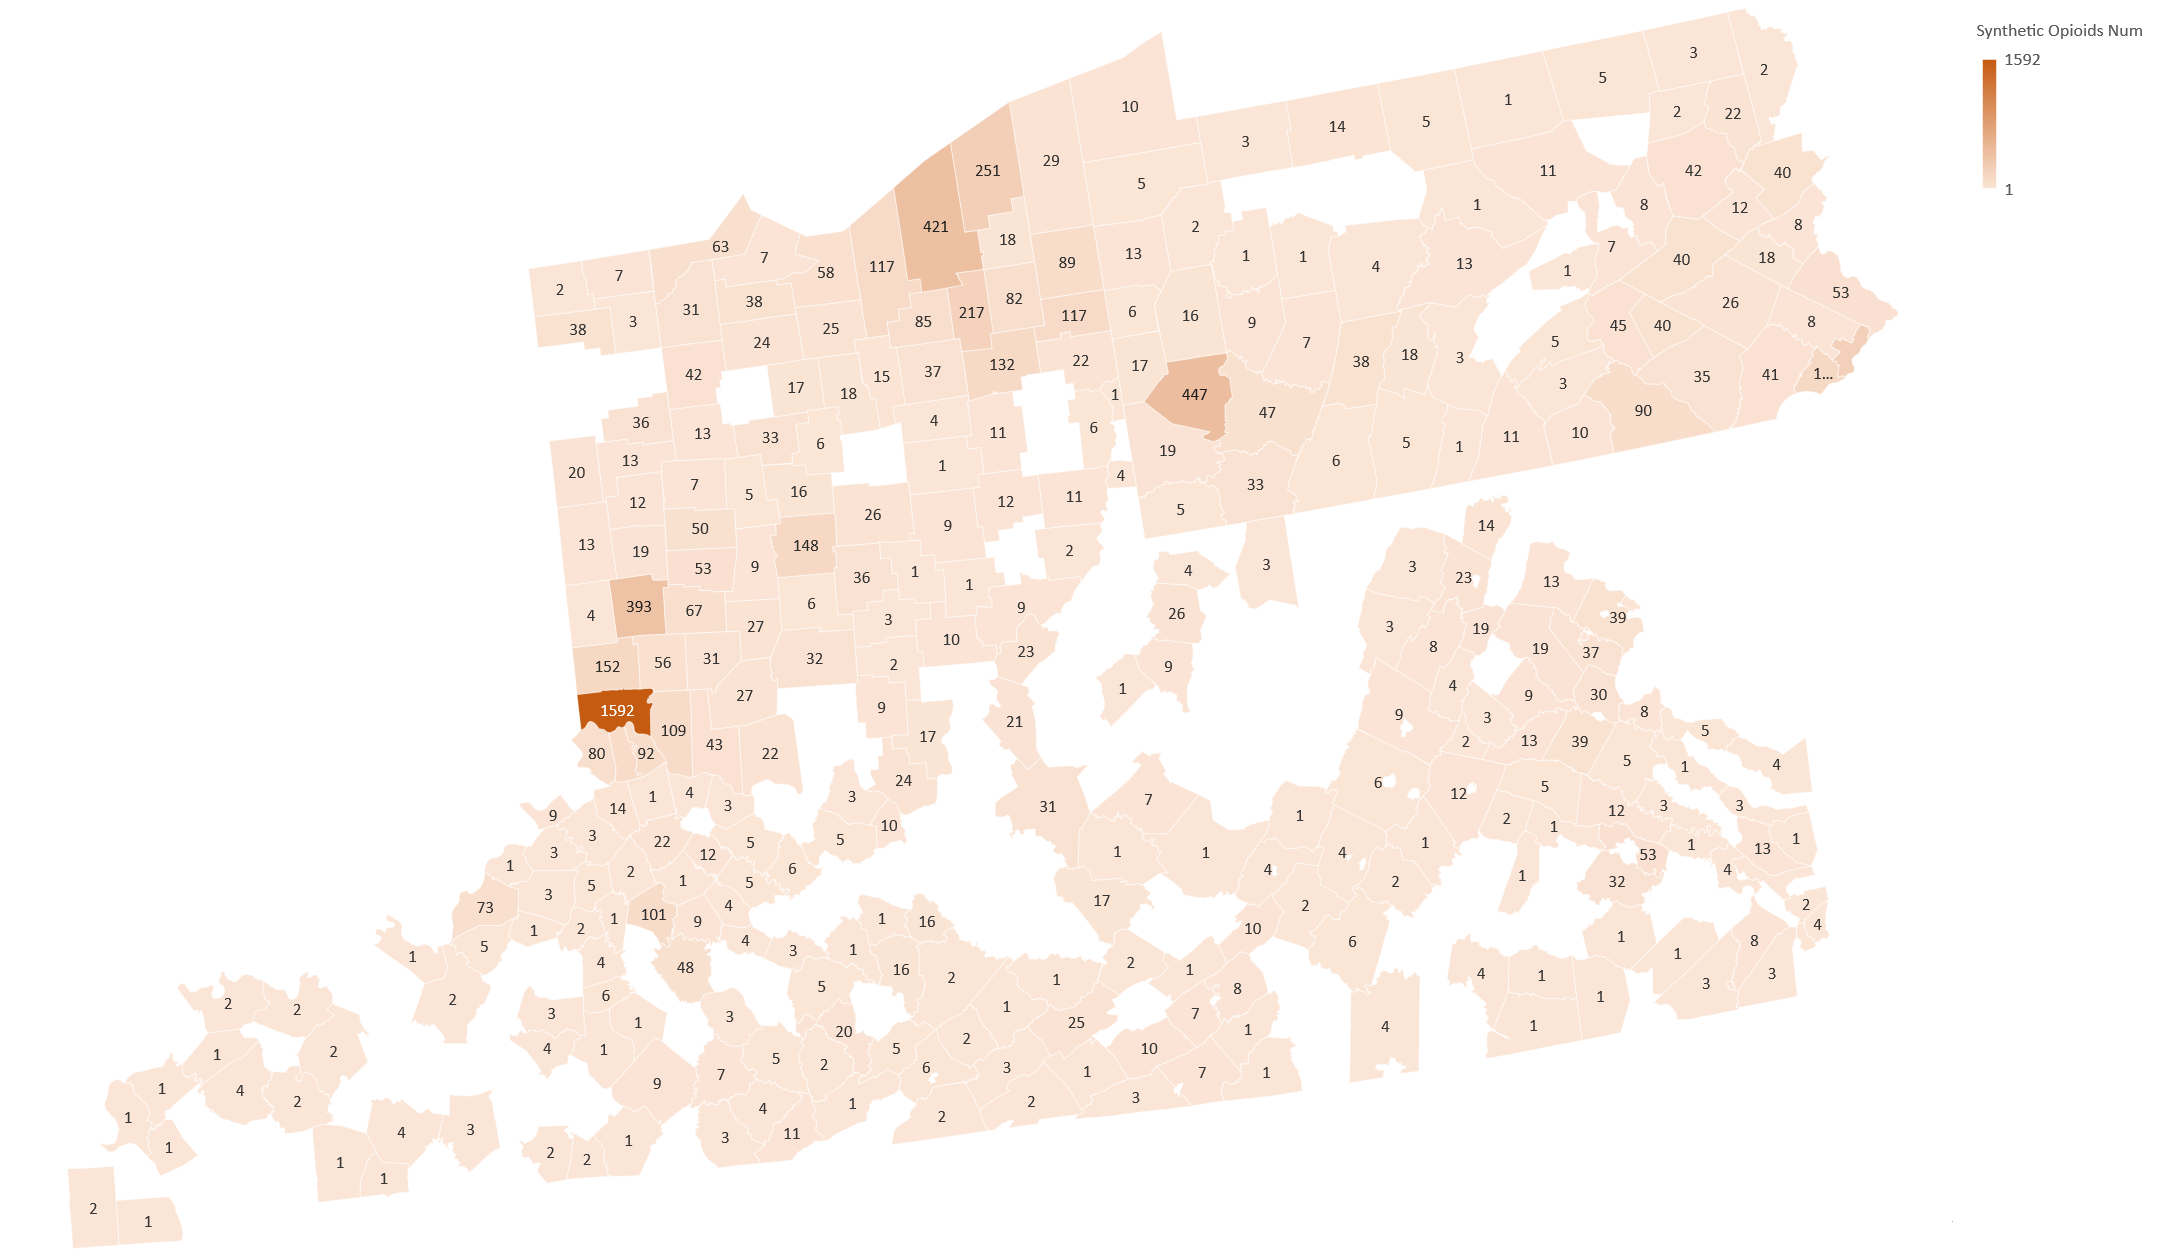
\includegraphics[width=\linewidth]{2015SYN.png}
     \caption{Synthetic Opioids Reports in 5 states in 2015}\label{S15}
  \end{minipage}
\end{figure}

\begin{figure}[H]
  \begin{minipage}{0.5\textwidth}
     \centering
     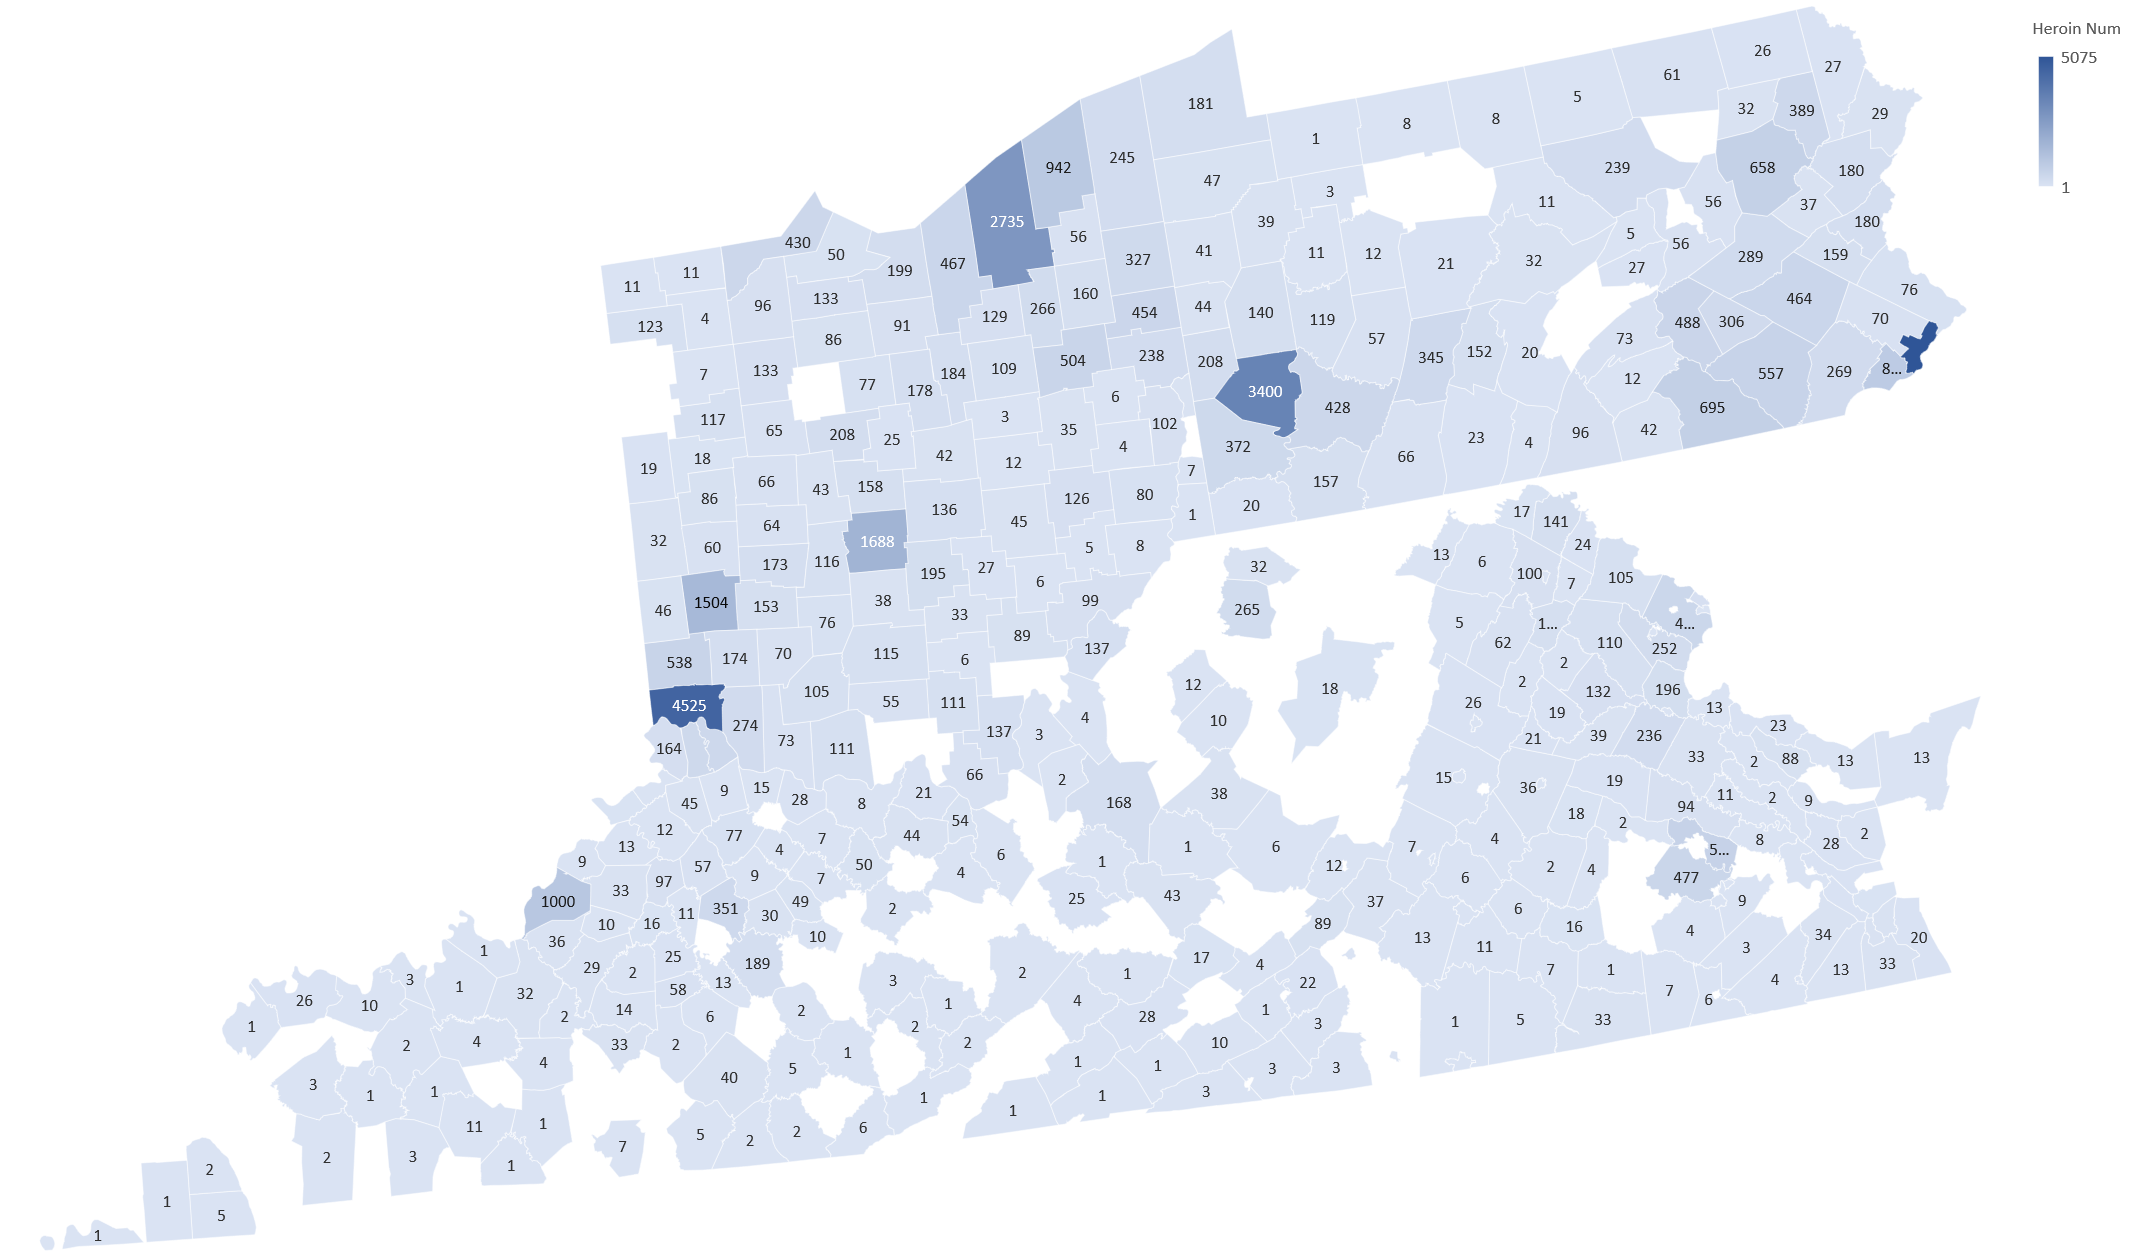
\includegraphics[width=\linewidth]{2016.png}
     \caption{Heroin Reports in 5 states in 2016}\label{H16}
  \end{minipage}%\hfill
  \begin{minipage}{0.5\textwidth}
     \centering
     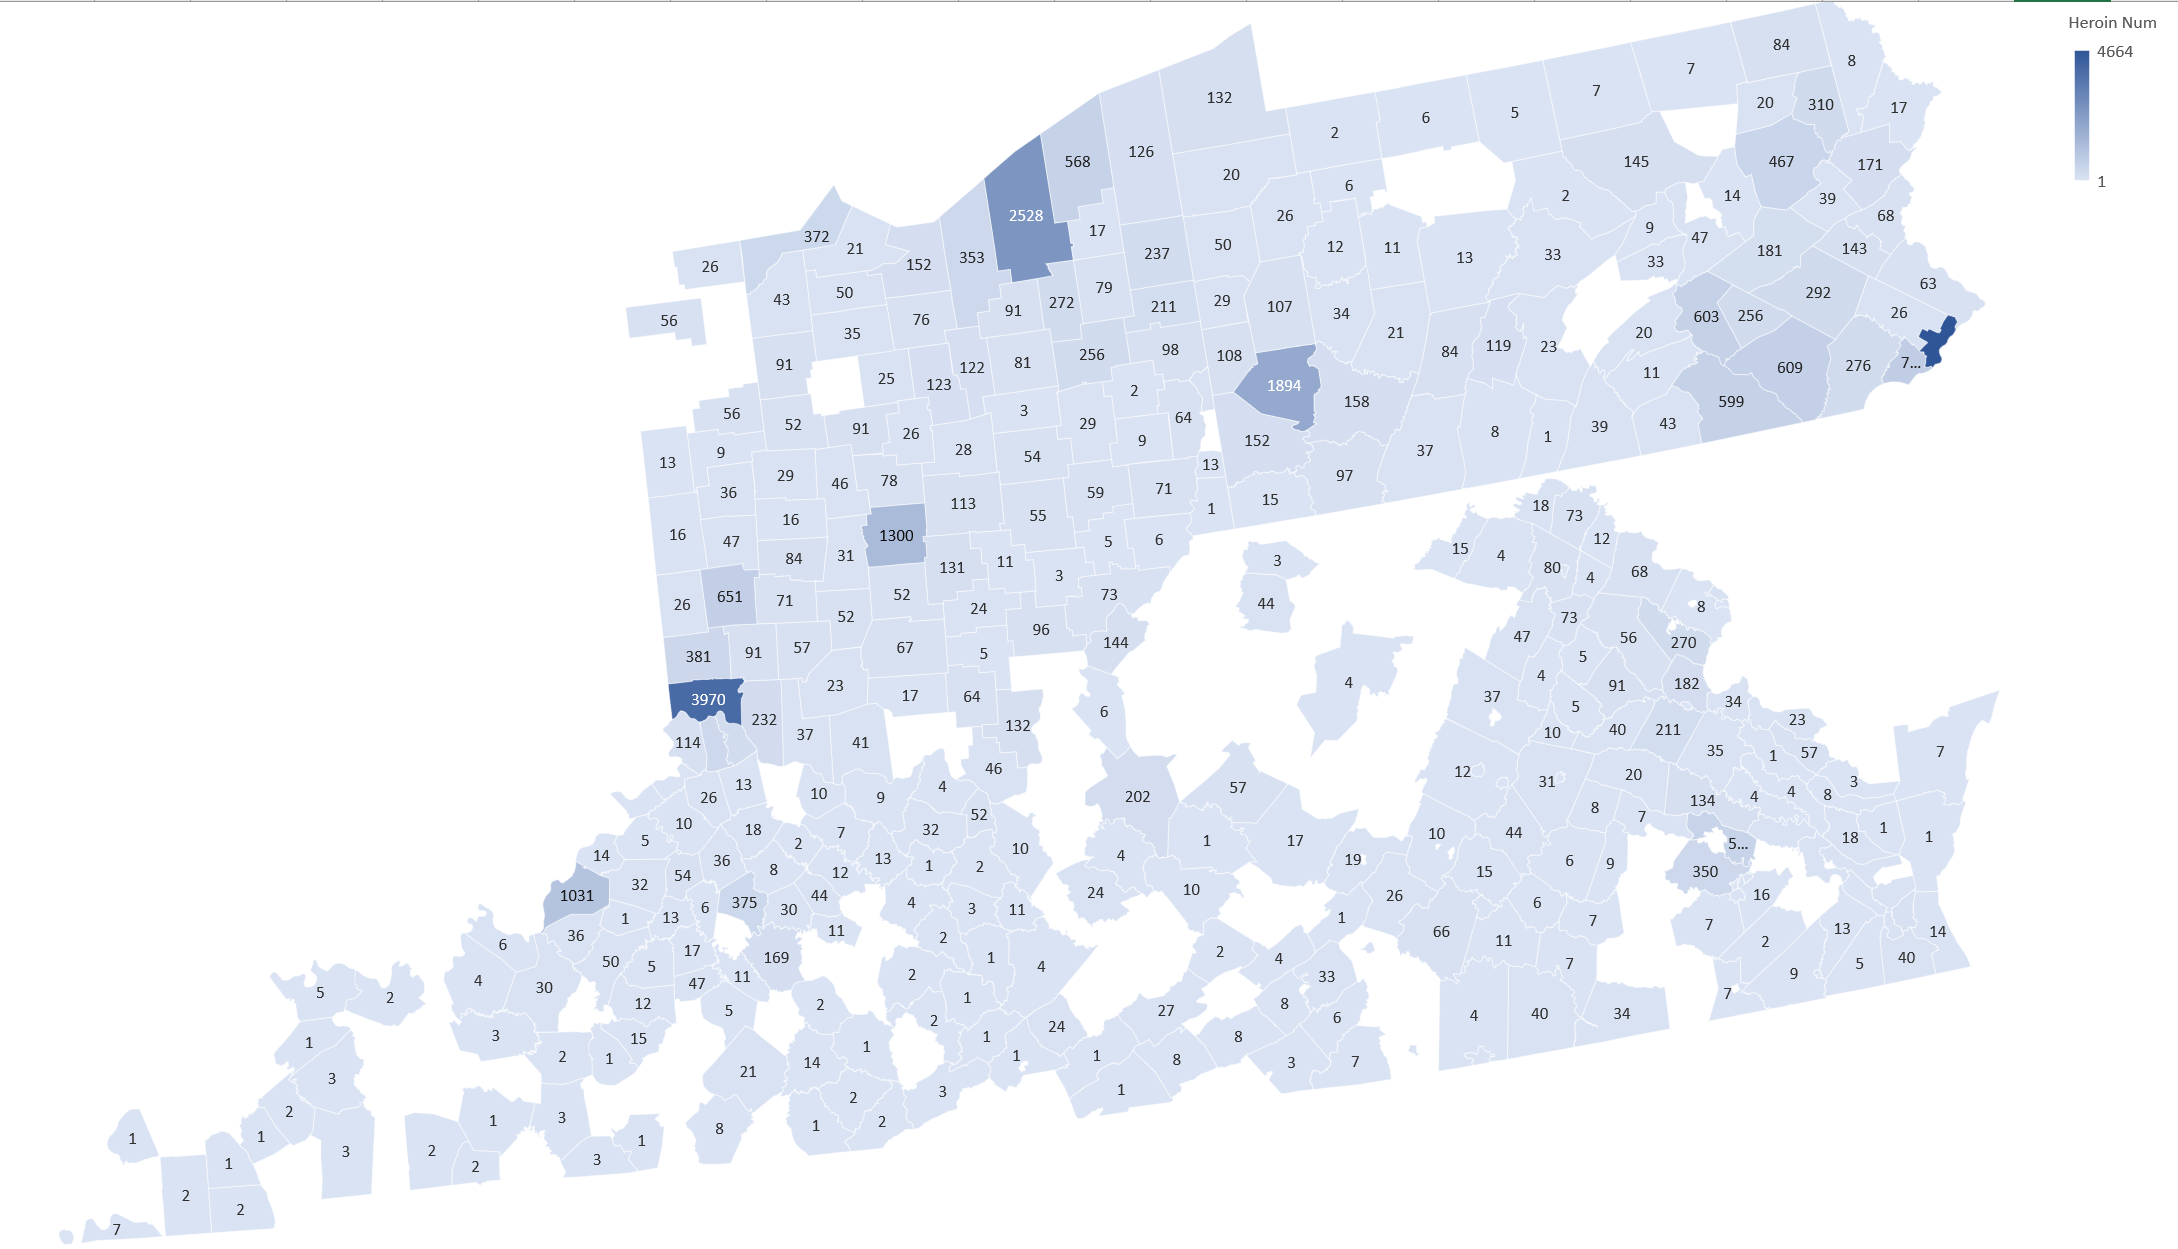
\includegraphics[width=\linewidth]{2017.png}
     \caption{Heroin Reports in 5 states in 2017}\label{H17}
  \end{minipage}
\end{figure}

\begin{figure}[H]
  \begin{minipage}{0.5\textwidth}
     \centering
     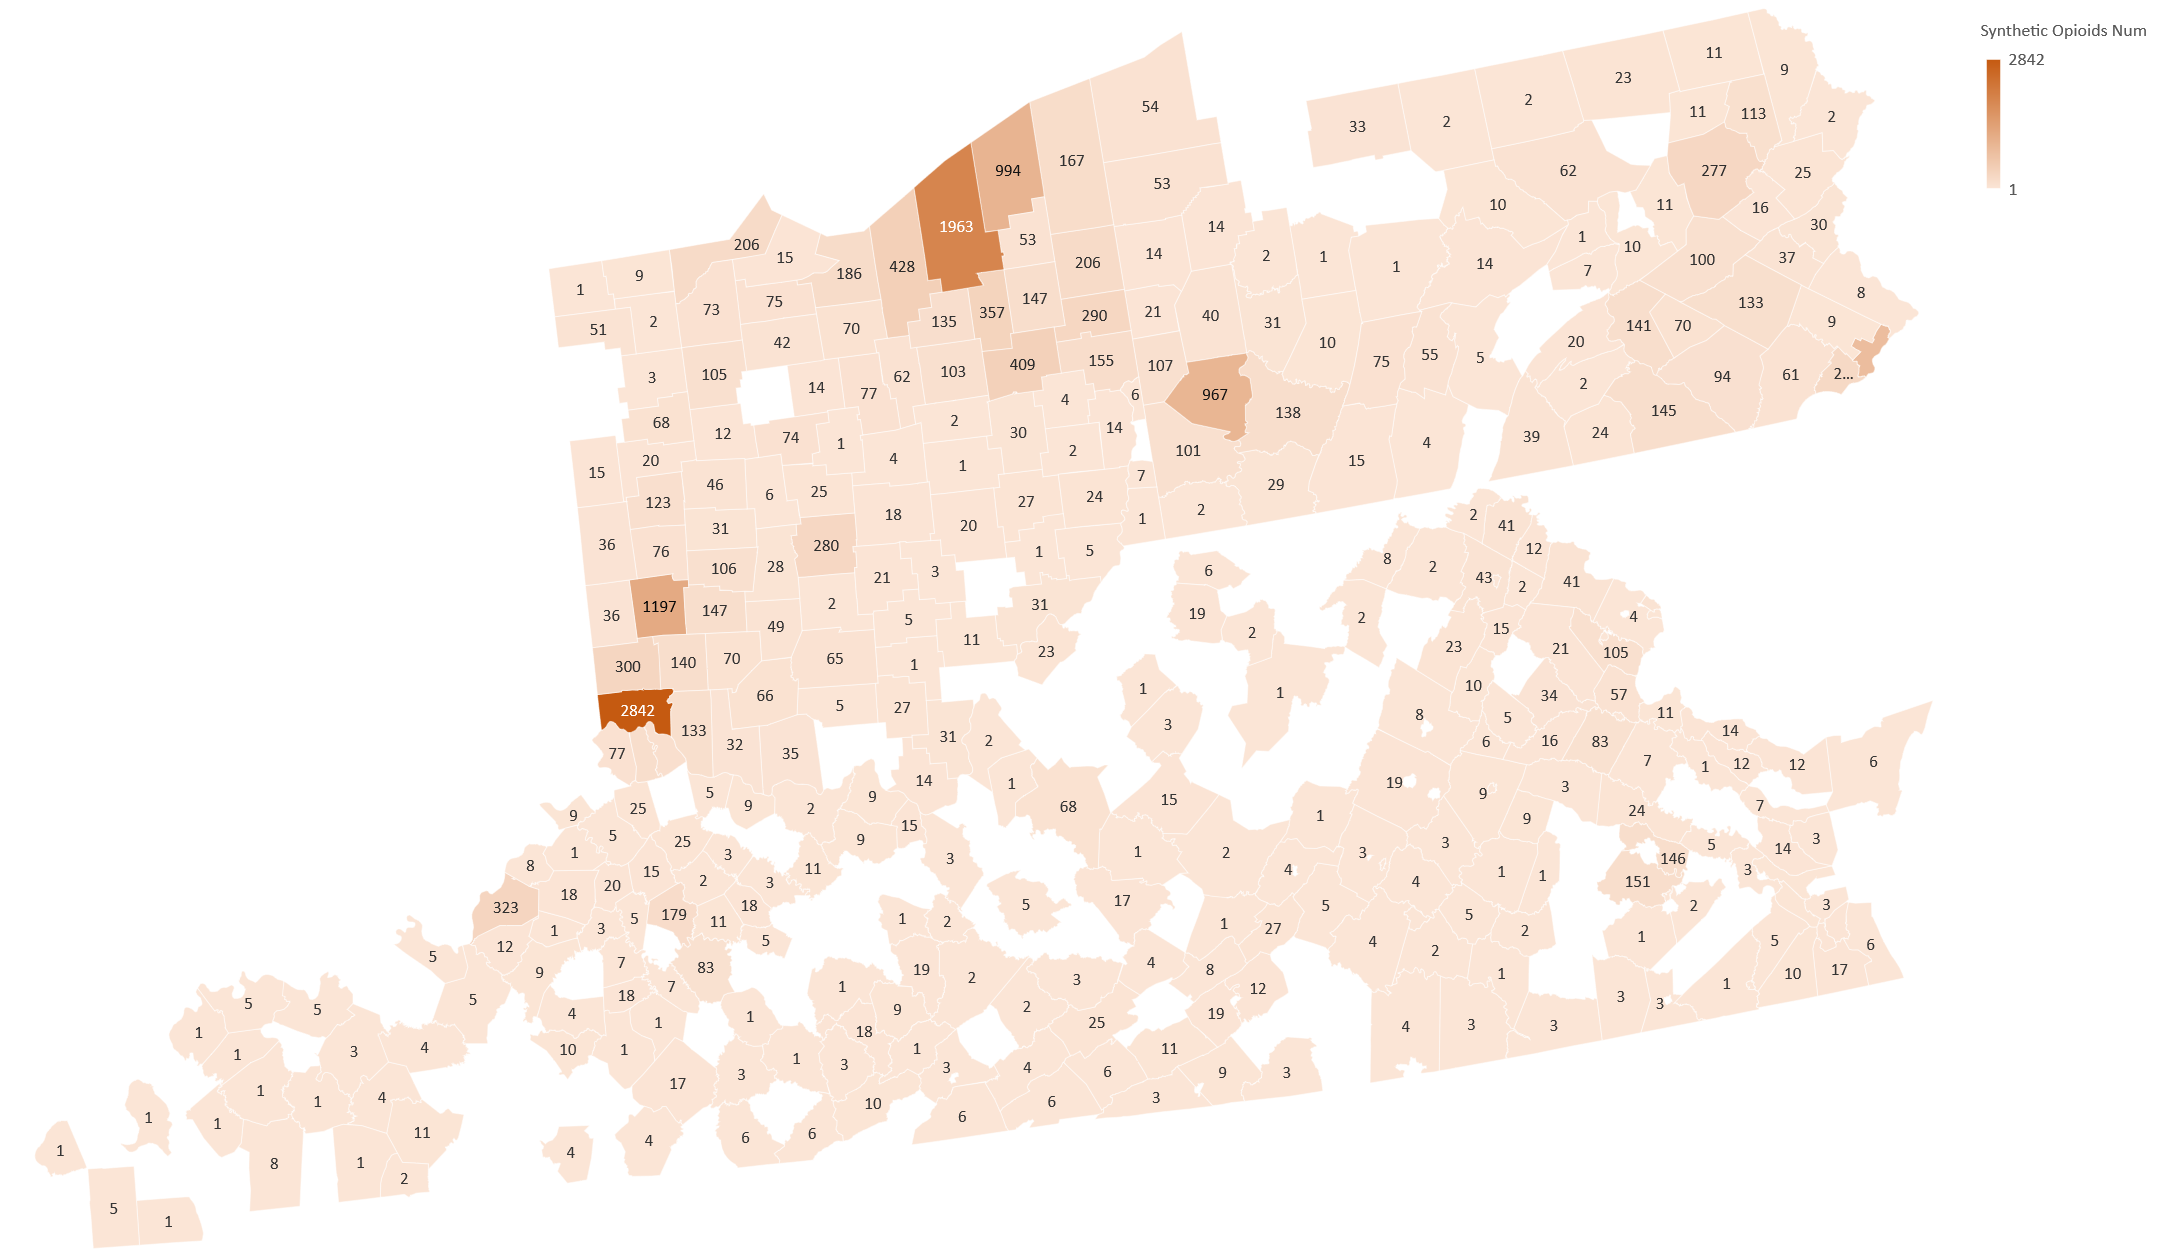
\includegraphics[width=\linewidth]{2016SYN.png}
     \caption{Synthetic Opioids Reports in 5 states in 2016}\label{S16}
  \end{minipage}%\hfill
  \begin{minipage}{0.5\textwidth}
     \centering
     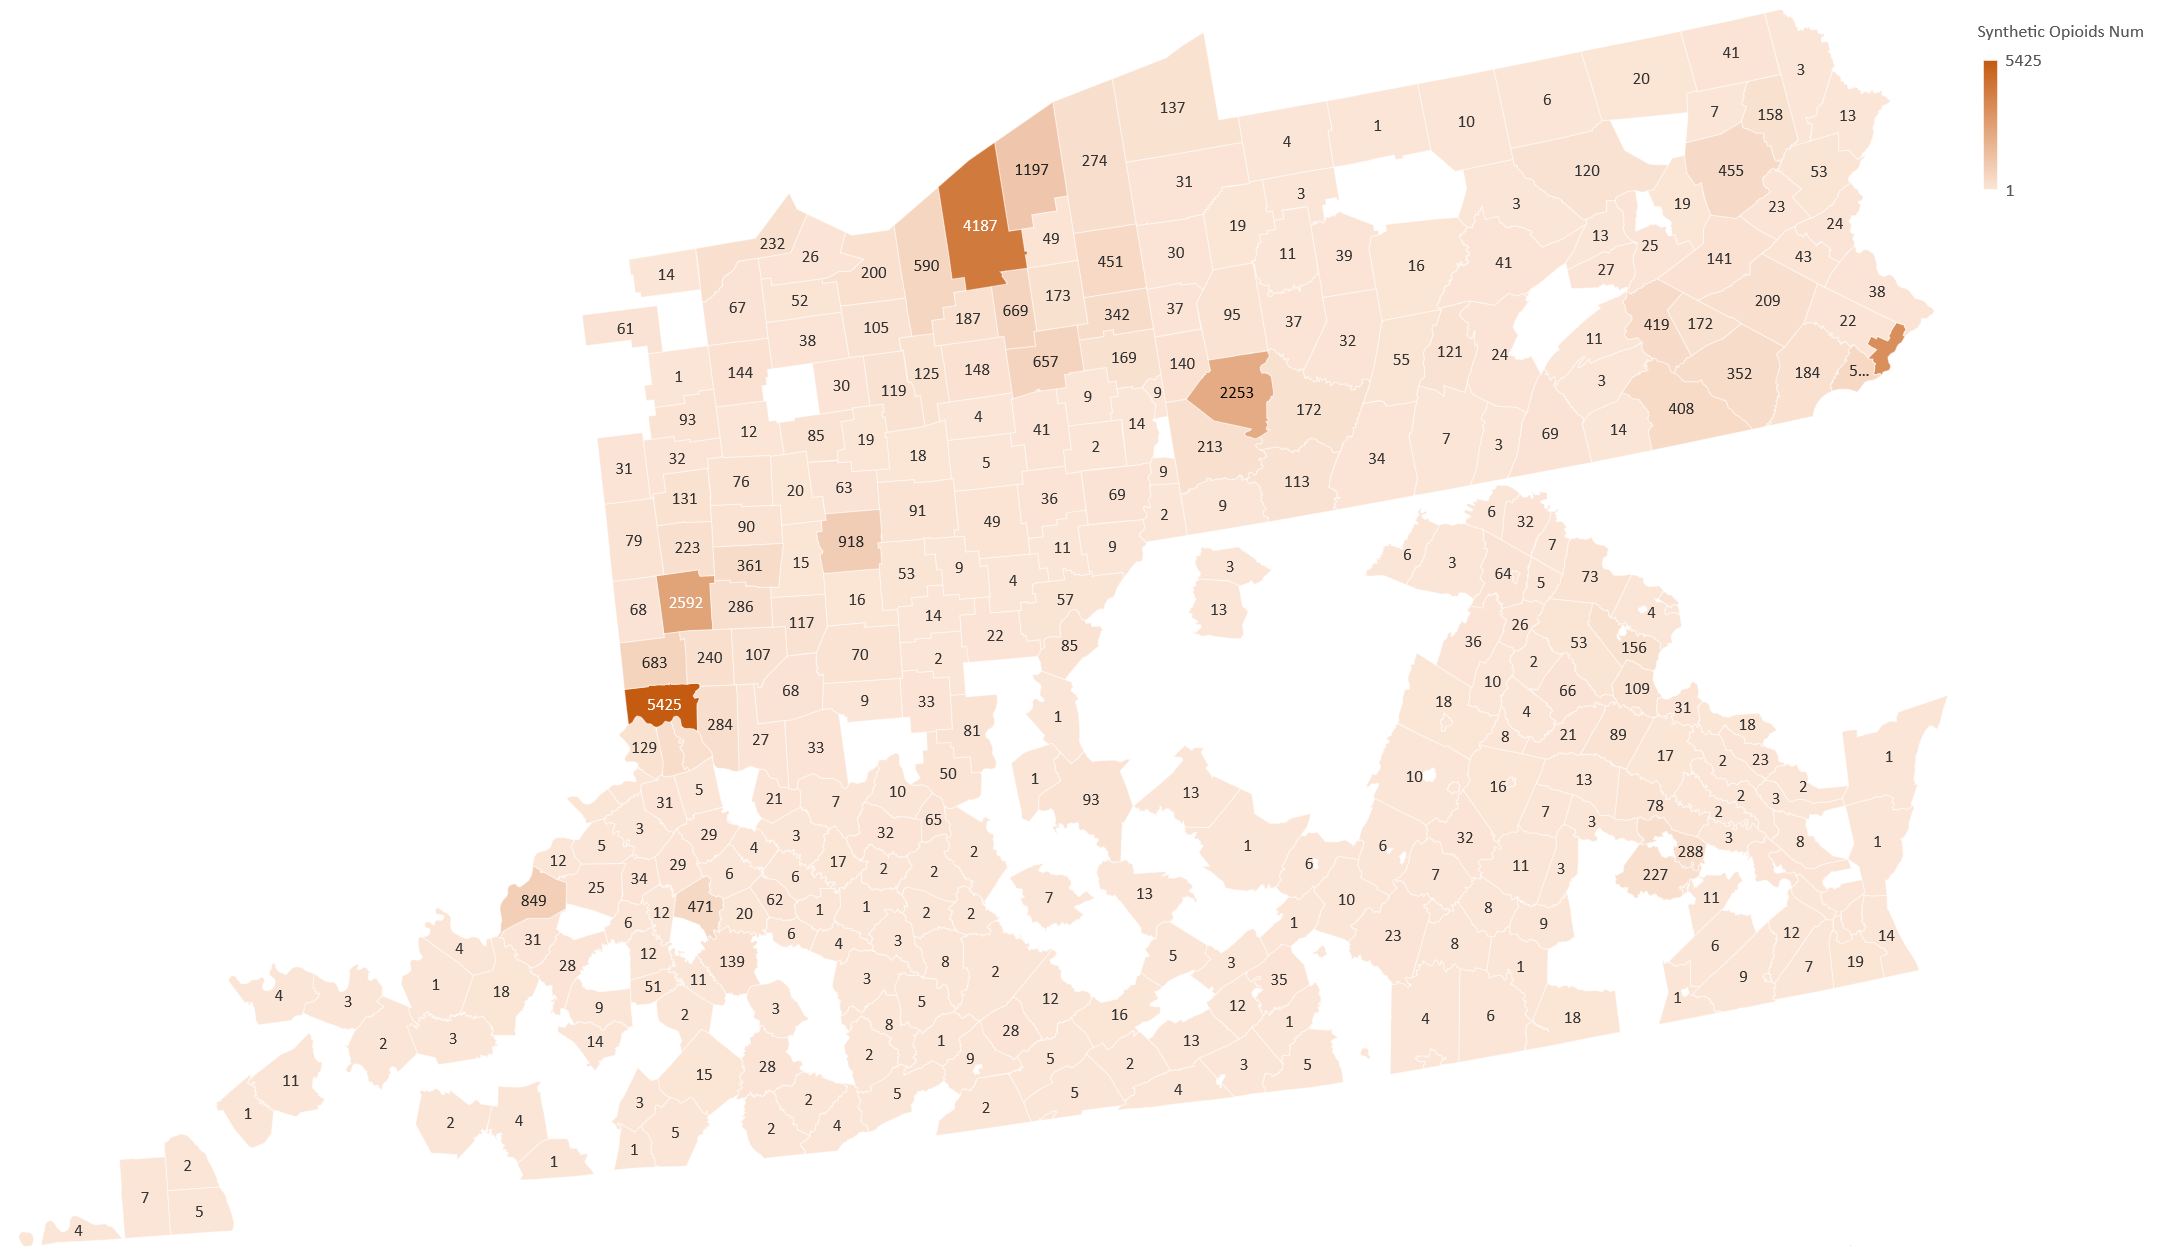
\includegraphics[width=\linewidth]{2017SYN.png}
     \caption{Synthetic Opioids Reports in 5 states in 2017}\label{S17}
  \end{minipage}
\end{figure}

%----------------------------------------------------------------
%---------------------END ADD IT BACK-----------------------------
%----------------------------------------------------------------

 \subsection{Cellular Automaton (CA) Model Framework}
% \begin{figure}[H]
%   \begin{minipage}{0.5\textwidth}
%      \centering
%      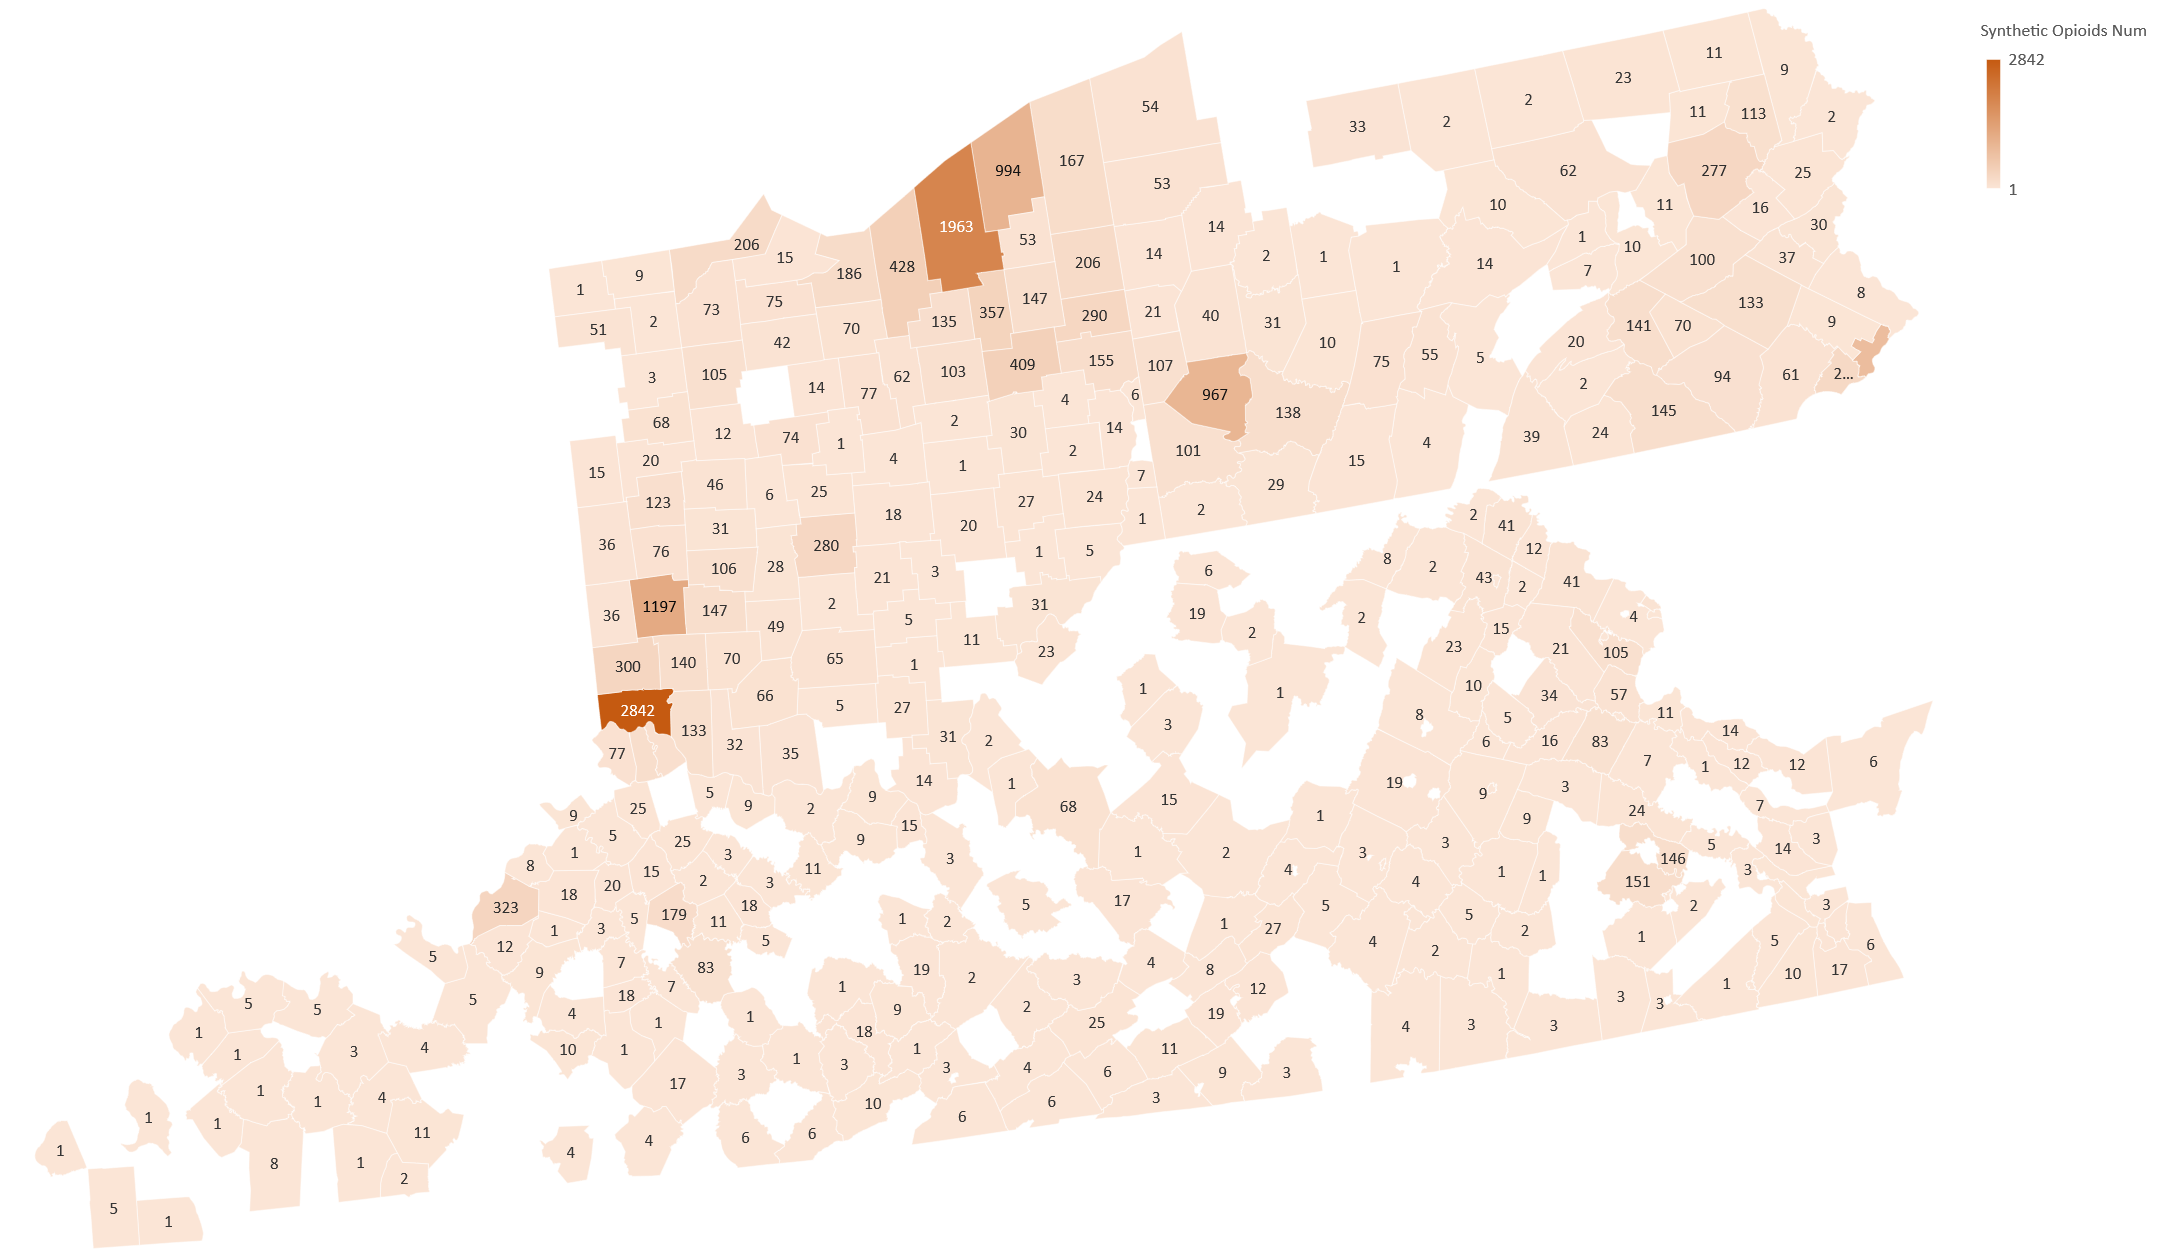
\includegraphics[width=\linewidth]{2016SYN.png}
%      \caption{Synthetic Opioid Reports in 5 states in 2014 2016}\label{S16}
%   \end{minipage}%\hfill
%   \begin{minipage}{0.5\textwidth}
%      \centering
%      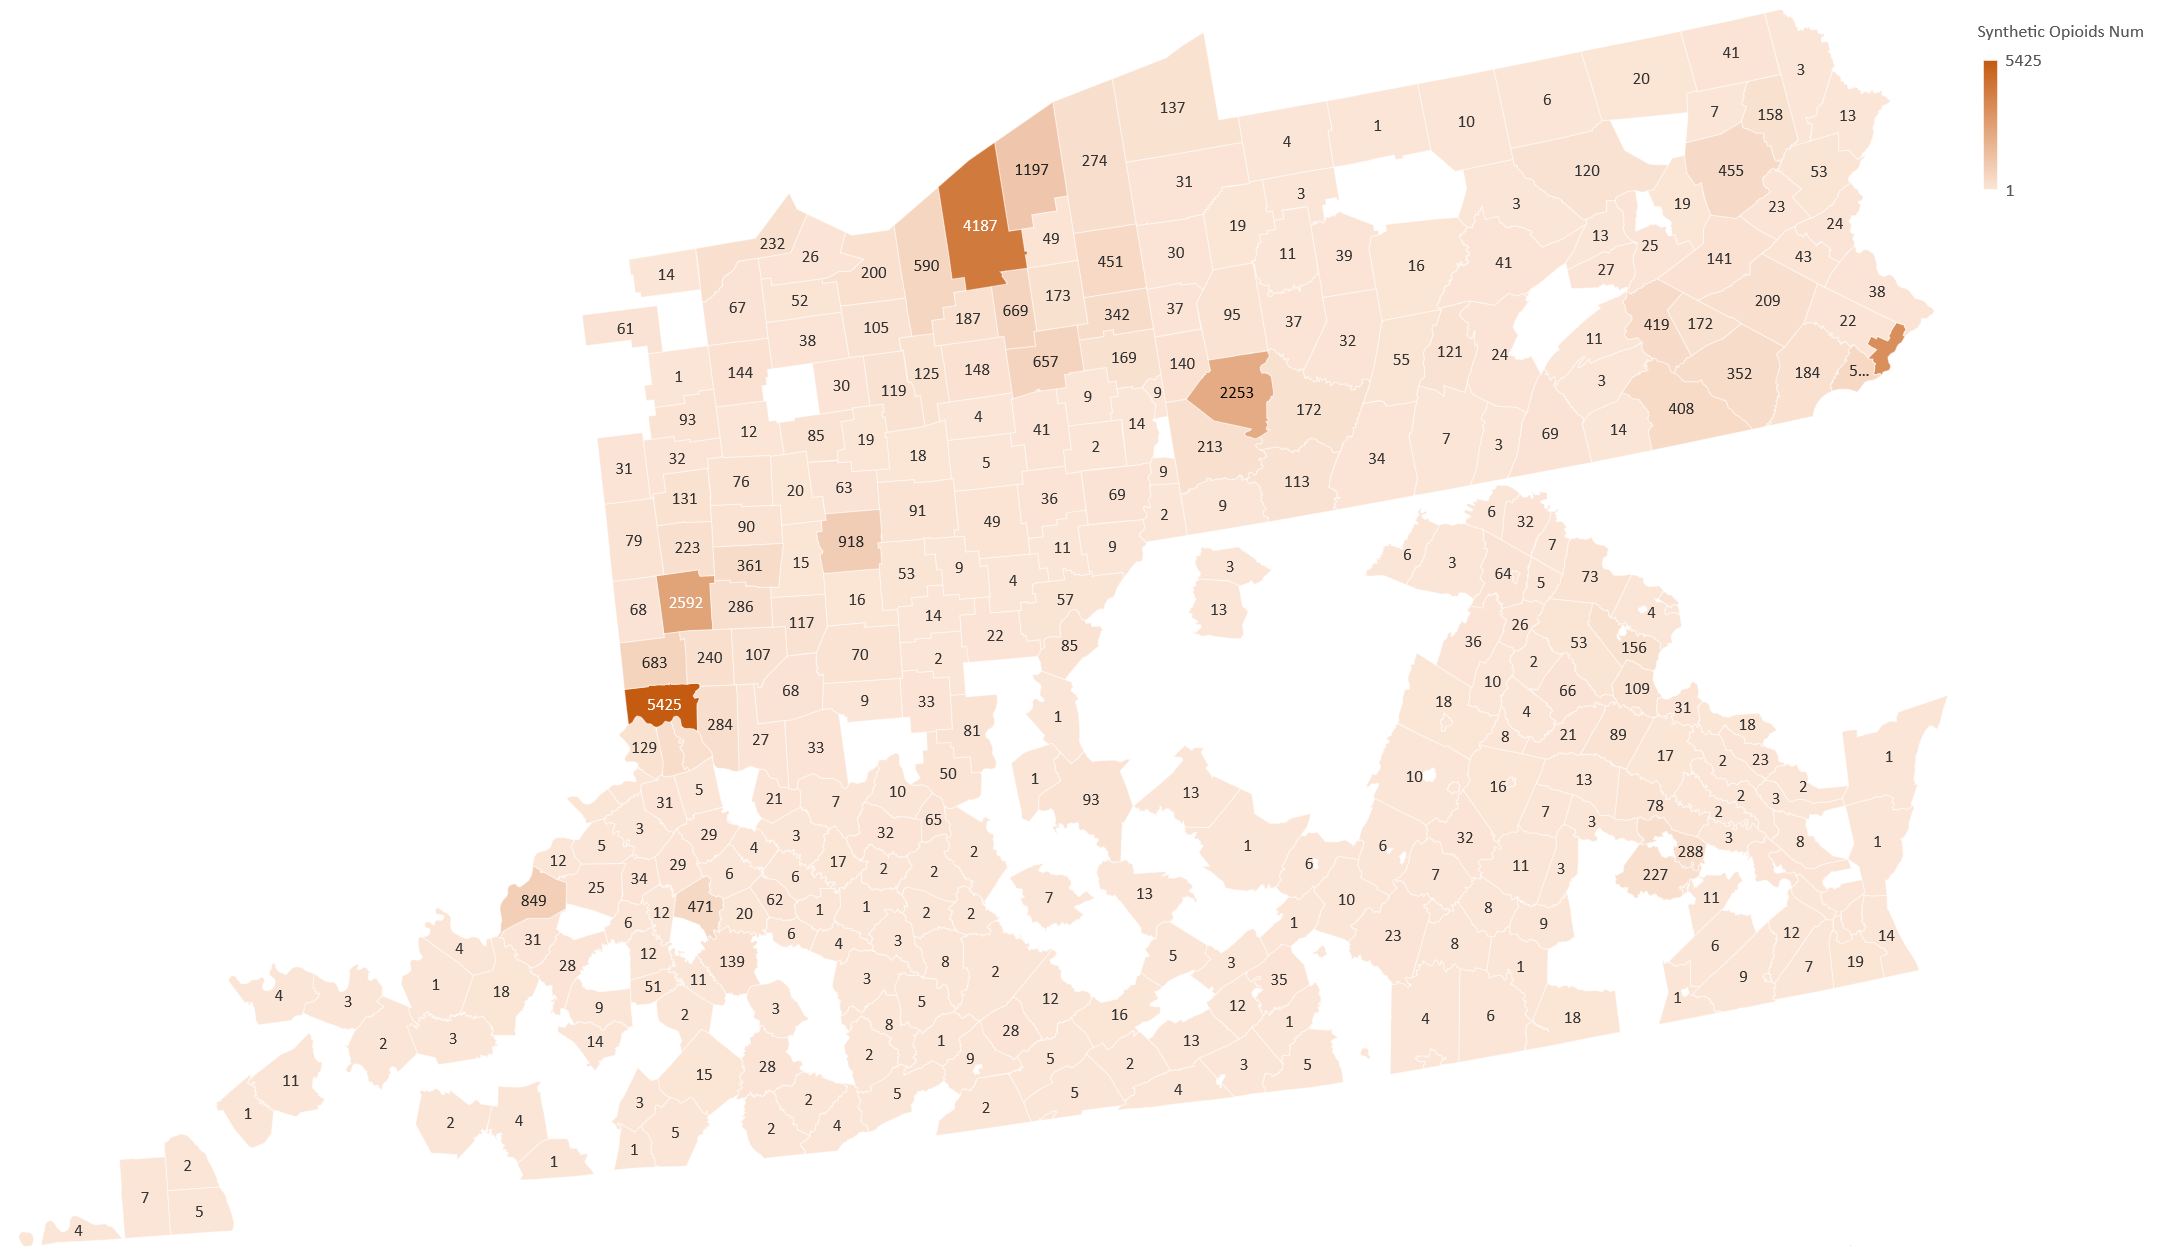
\includegraphics[width=\linewidth]{2017SYN.png}
%      \caption{Synthetic Opioid Reports in 5 states in 2014 2017}\label{S17}
%   \end{minipage}
% \end{figure}

%In this model, we assume a constant size of population with recruitment and non-illicit-related death rate at time $t$ given by $\mu$. We separated the total population into several groups, including susceptible individuals, light and heavy drug users, people with mentally illness because of drugs, and detected illicit drug users.

%\begin{align}
%    N(t) = S(t) + I(t) + I_a(t) + M(t) + R(t),
%\end{align}
%~\\
%Then we assume that susceptible individuals acquire illicit drug use habits at rate \begin{align}
%    \lambda = \beta (I + \kappa I_a)
%\end{align}
%~\\
%The model then takes the form \begin{align}
%\begin{split}
%    \frac{dS}{dt} &= \mu - \lambda S - \mu S, \\
%    \frac{dI}{dt} &= \lambda S - (\alpha + \gamma + \sigma + \mu + \psi)I, \\
%    \frac{dI_a}{dt} &= \alpha I - (\rho + \phi + \mu + d)I_a, \\
%    \frac{dM}{dt} &= \sigma I + \phi I_a - (\epsilon + \mu + \delta)M, \\
%    \frac{dR}{dt} &= \gamma I + \rho I_a + \epsilon M - (\mu + \omega)R
%\end{split}
%\end{align}
%~\\
%Put equations (3) in the closed set, we will have \begin{align}
%    \Omega = \{(S, I, I_a, M, R) \in %\mathbb{R}^5_+ : 0 \le N \le 1\},
%\end{align}
%~\\
%where $\Omega$ is positively invariant with respect the the above equations (2).

For the purpose of our model, we decide to use a 2-D cellular automaton system. In spite of the simplicity of their structure, the Cellular Automaton(CA) we use can perform quite complex trend and involvement of the drug crisis that we are going to analyze if given enough constraints and parameters.\\
A cellular automaton (referred as CA in the following text) is characterized by the following five properties:
\begin{enumerate}
\item the number of spatial dimensions ($n$);
\item the width of each dimension ($w$), $w_k$ is the width of the $k$th dimension where $k = 1,2,...,n$;
\item the width of the neighborhood of each cell $(d)$. $d_k$ is the width of the neighborhood of the $k$th dimension;
\item the local status of each of the CA cells;
\item the CA rule, which is an arbitrary function called $F$.
\end{enumerate}
Notice that the change of state of a specific cell from time $t$ to $t+1$ is computed according to $F$. $F$ is a function of the state of itself as well as all the neighborhood cells at time $t$. 
~\\
\subsubsection{CA Formation for this problem}
Our CA model is a 2 dimensional grid where the width of the two sides are taken to be equal, namely $w_1 = w_2$. Each cell in the grid represents a county according to the geographic information on map such that the location and neighborhood information is well-preserved in this grid. Although not accurate and non-realistic, for this specific problem, we are restricting the inter-county communication only to the neighborhood counties, that is, a county can only be influenced by its 8 neighbors, namely on the top, left, right, bottom, top left, top right, bottom left and bottom right. We will discuss the impact of global communication in later sections.

At the initial time, we assign a initial state to each of the cell in the grid according to a specific local rule. This rule is defined as following:
~\\
The state $C_{i,j}^t$ of the $(i,j)$ CA cell at time $t$ is
\begin{equation}
   C^t_{i,j} = \{S_{i,j}^t,\text{ INF}^t_{i,j}\},
   \label{state}
\end{equation}
where\\
$\text{INF}^t_{i,j}$ is a ``infectious flag'' with only binary values 0 and 1,\\
$S_{i,j}^t$ is the number of the certain opioid reports during year $t$.\\
\subsubsection{CA Rule}
The value of the flag indicates whether there are drug reports from this state at time $t$ or not. If $\text{INF}^t_{i,j} = 1$, then the $(i,j)$ cell is a drug infected county.[2]
~\\
The transition of the state of each cell each time step is done according to the following function:
\begin{align}
\begin{split}
    S_{i,j}^{t+1} &= (1 + (\rho \cdot [S_{i,j}^t > \kappa]))\cdot S_{i,j}^t \\
    &+ k\cdot (S_{i-1,j}^t + S_{i,j-1}^t + S_{i,j+1}^t + S^t_{i+1,j})\\
    &+ l \cdot (S_{i-1,j-1}^t + S_{i+1,j-1}^t + S_{i-1,j+1}^t + S^t_{i+1,j+1})
\end{split}
\label{CArule}
\end{align}
where\\
$\kappa$ is the threshold value for the annual number of the certain opioid reports within a county,\\
$[S_{i,j}^t > \kappa] \in \{0,1\}$. If $S_{i,j}^t > \kappa$ is true, $[S_{i,j}^t > \kappa]=1$. If it is false, $[S_{i,j}^t > \kappa]=0$.\\
$\rho$ is the self-increasing rate of a county if the number of the certain opioid reports is larger than $\kappa$,\\
$k$ is the coefficient that represents the effect of the neighbors sharing a side with the cell,\\
$l$ is the coefficient that represents the effect of the diagonal neighbors of the cell.\\

\subsection{Neighborhood Influence}
The state of the cell $(i,j)$ at time $t+1$ depends on both within the county and the state of all the 8 neighbors around it as shown in Figure \ref{grids}. 

But the neighborhood influence is at a different rate since they have different boarder lengths. The effect of the adjacent neighbors, namely, $(i-1,j), (i+1,j), (i,j-1), (i,j+1)$ is multiplied by $k$ and the effect of the diagonal adjacent neighbors is multiplied by $l$. Notice that the cells with common sides have more connection with $(i,j)$, while the other four cells which are on the corners would have less connections and thus have less influence on the central one. Therefore, it is always the case that $k > l$.

On the other hand, there are influence within each county, too. Apart from the influence from the neighbors, the size of drug users would increase within the county itself if no severe regulation is posted. Therefore, $\rho$ is the self increasing rate of a county if the drug community in that county is larger than some threshold value $\kappa$. 
\begin{figure}[H]
    \centering
    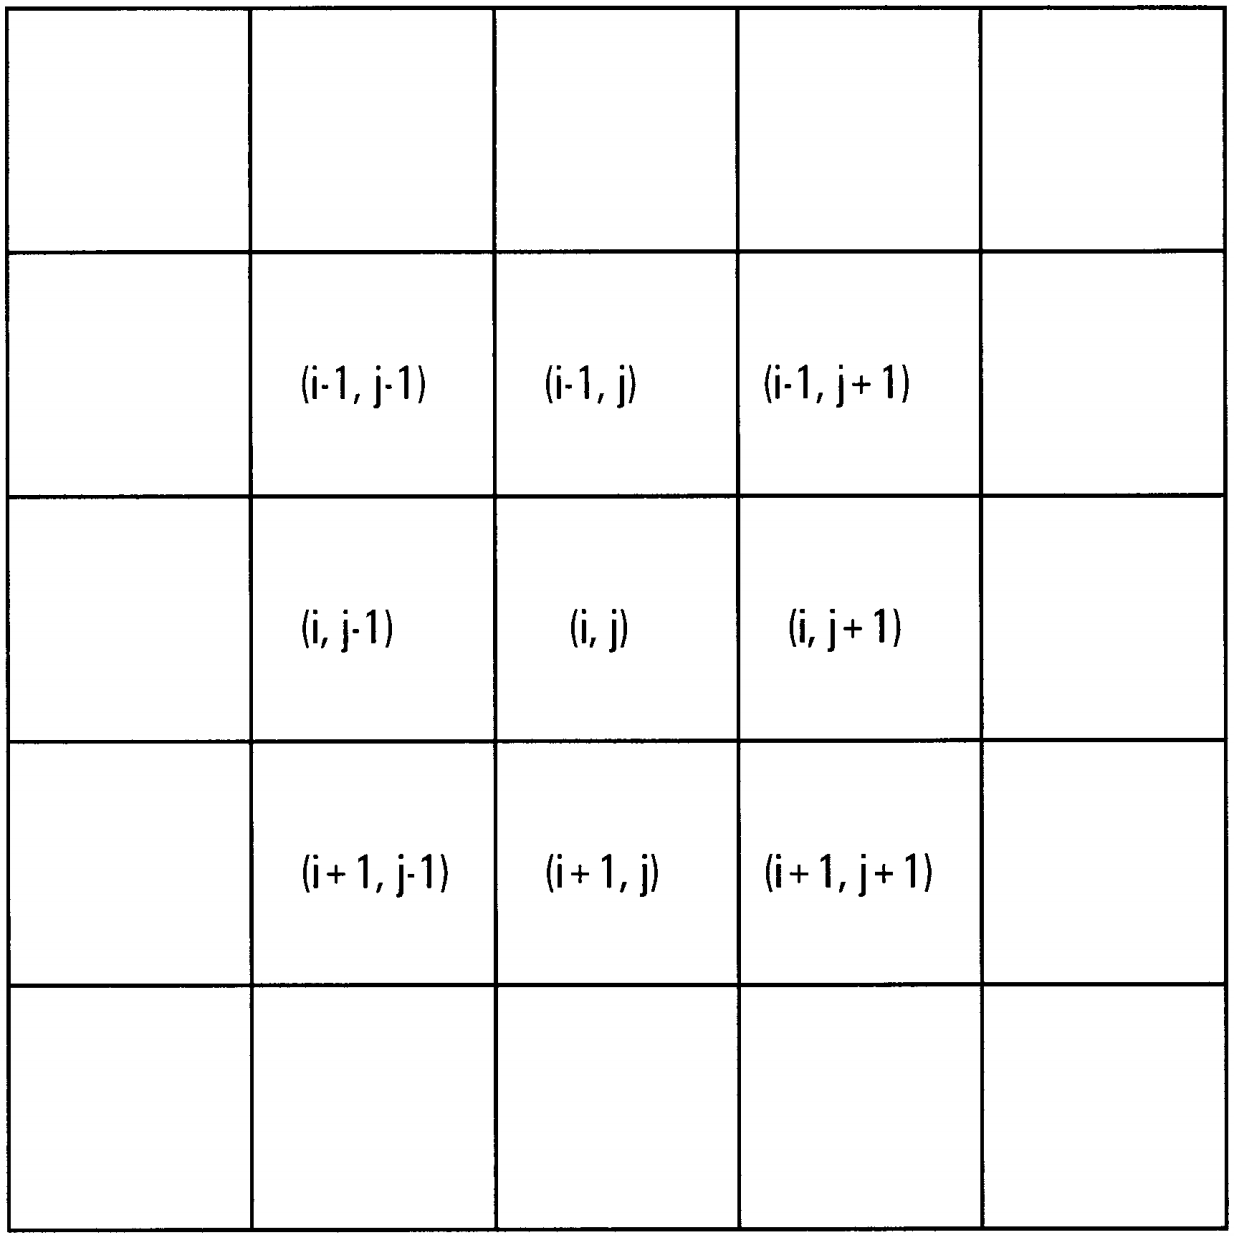
\includegraphics[width = 0.5\textwidth]{grids.png}
    \caption{Neighborhood cells of the $(i,j)$ cell}
    \label{grids}
\end{figure}



\subsubsection{Possible Problems on this model}
Notice that this model was based on the assumption that no drug users could actually recover from their addiction and little restriction was pushed upon. Therefore, the number of reports within our model will always be increasing instead of decreasing since we do not have the mechanism of control the number of drug users.

\subsection{CA on Data}
Based on the model described above, we applied it to the real data we are given. In order to successfully apply this model, we first partitioned the map of the 5 states into grids where each cell has roughly the same size as the counties on the map we generated. According to the cell each county lands on, we can assign a cell to it. In this case, we can express each county as a cell and perform the CA algorithm on the county easily. An example of our partition is figure \ref{partition}:

\begin{figure}
    \centering
    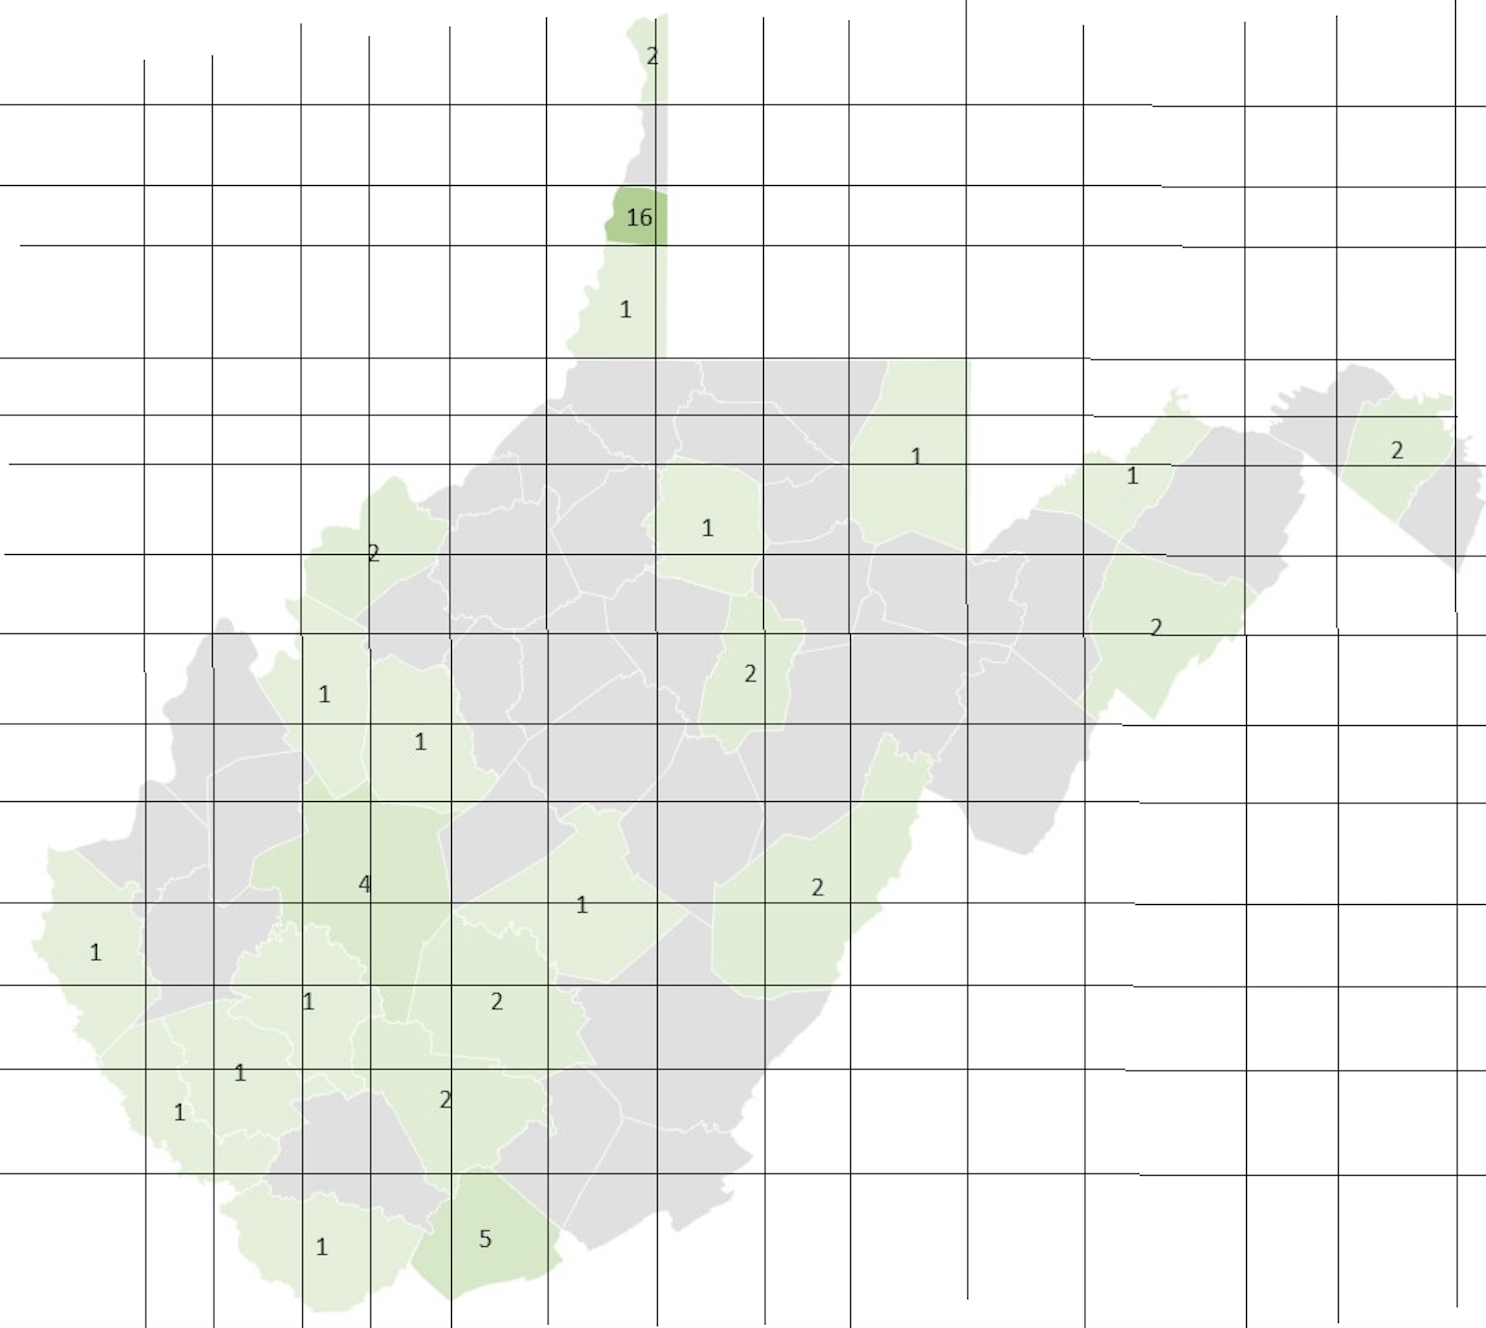
\includegraphics[width = .9\textwidth, height = 10.5cm]{gredEg2.png}
    \caption{Sample partitioning for the state of West Virginia}
    \label{partition}
\end{figure}

One thing we had to take care was the inaccuracy of this assignment. There are a lot of incidents where we have more than 1 county land in the same cell or we have counties that lands across several cells. One effort we made to improve this situation was to personally observe the relationship of these stacking positions and try to assign them the best cells such that they still well-preserve the geographic properties and the relative location of these counties.

Now we have our 2-D array of cells ready for the model to run.

\subsubsection{Model Initialization}
Before the simulation of the model, we have to initialize the cell states such that we have a initial condition for the model to run. To achieve this, we filtered the data both using Python and Excel and found the number of heroin and synthetic opioid reports separately. %Could delete this%
Then we filled in these values into the cell of each county and got the initial state of the model. 

The next thing we did was to find the correct unknown coefficients in equation \ref{CArule}, namely $\rho, \kappa, k$ and $l$, such that we can use it to actually predict the patterns after the year 2017. Although we didn't manage to come up with a method to actually find these values by regression or machine learning, we still got pretty satisfactory results by trying reasonable values by hand.

First we decided that roughly 
\begin{equation}
    \kappa = 20
\end{equation}
 since an annual report under 20 might not be significant enough to form a mature drug community which could grow by a certain rate annually. Also from the raw data we found out that almost all counties with drug reports under 20 in year 2010 did not evolve into larger drug community in year 2017. 

We then tried to find out a reasonable range for $\rho$, which is the internal increasing rate of a large enough county which has more reports than the $\kappa = 20$. In order to get a reasonable number for $\rho$, we wrote a small program in Python to find out the average annual increasing rate for all counties within the 7 years. For all counties with more than 20 heroin and synthetic opioids reports or with a 7-year difference greater than 20, we compute
\begin{equation}
 \left(\frac{r_{2017}}{r_{2010}}\right)^{\frac{1}{7}}  
\end{equation}
and take the average. Here, $r_{2017}$ is the number of reports in 2017 while $r2010$ is the number of reports in 2010. This method might not be accurate enough but it is just providing us with a rough range of the actual value $\rho$. In turned out that the average we computed was $1.038$, it follows that we roughly got the value 
\begin{equation}
    \rho = 1.038-1 = 0.038.
\end{equation}

In order to find the value for $k$ and $l$, we tried several different values and then compared it with the 2017 map to see how well they behaved.

It turns out that, the model yields the best fit with the actual data in year 2017 when
\begin{align}
  k &= \frac{1}{\max (R(s))}  \\
  l &= 0.7 \cdot k
\end{align}
  
where $R(s)$ is the set of the number of county drug reports in a certain state $s$. That is, when $k$ is the reciprocal of the maximum report number is a certain state, the model performs the best. 

\subsubsection{Modified Model Looking for the Starting Position}
In order to trace backwards for the starting point for each state, we modified our model such that all impacted are switched to negative. That is, all neighbors are negatively impacting the middle cell and the middle cell is also decreasing at a certain rate.

Specifically, we use basically the same model function $F$ but with different coefficients. We have chosen
\begin{equation}
\begin{split}
\rho_{back} &= \frac{1}{1.038} - 1 = -0.037\\
k_{back} &= -k\\
l_{back} &= -l\\
\kappa_{back} &= 20
\end{split}
\label{backwards}
\end{equation}
We have made $\kappa = 20$ since when going backwards, there are a lot of counties starting from a very low number, namely, lower than 20. If the threshold is too large, the model would have no meaning. The other coefficients are just the reciprocal of themselves. In this case, we can trace back for the first appearance within each state.


%%%%%%%%%------------------------
%--------------------------------------
%-----------------------------------
%--------End of section 3-----------------
%------------------------------------
%--------------------------------------
%---------------------------------------


\section{CA Model with socio-economic data}
There are various hypothesis trying to explain how the opioid-use get to such a high level. Many scholars promote the effect of family support. For instance, United Nations Office on Drugs and Crime(UNODC) states that family dynamics is one of the most important factor on whether kids from these families would fall into drug addiction. According to UNODC, household stability, income and employment may boost the stress of the family and push familiy members to look for "solutions", which is possibly using drugs.[?]\\ %%%%%fill the reference number
In this part, we examine the U.S. Census socio-economic data provided to check which factors in the list has a relative substantial influence on the current opioid-use level. Then we improve the model,i.e. Equation \ref{state}, from previous part by implementing the factors into the function for more precise outputs. On the one hand, we gain a better model that operates more closely to real-life progress. On the other hand, we get to realize how some ordinary socio-economic situation around us might lead to such a social security crisis.\\
\subsection{Obtain the Influential Factor}

U.S. Census socio-economic data provides a detailed table about different household status such as marital status, fertility, as well as grandparents raising children or not. We examine by plotting the data of each county in accordance with the total number of drug reports in that county to see if the peak points of the total number of drug reports meet some critical points in the graph of socio-economic data. \\
We simply choose four significant high peak points in the graph of total drug reports county as our representative points to test the factors, the counties of which are Philadelphia in PA, Allegheny in PA, Montgomery in OH, and Hamilton in OH. We color-coded each points that Philadelphia is in red, Allegheny is in yellow, Montgomery is in green, and Hamilton is in brown. The corresponding points in the three socio-economic graphs are colored the same color in regard with the location.\\
The following graphs showing the data that meets the condition to be our three influential factor,responsibility of grandparents taking care of grandchildren, education degree, and marriage experience.\\

\begin{figure}[H]
    \centering
    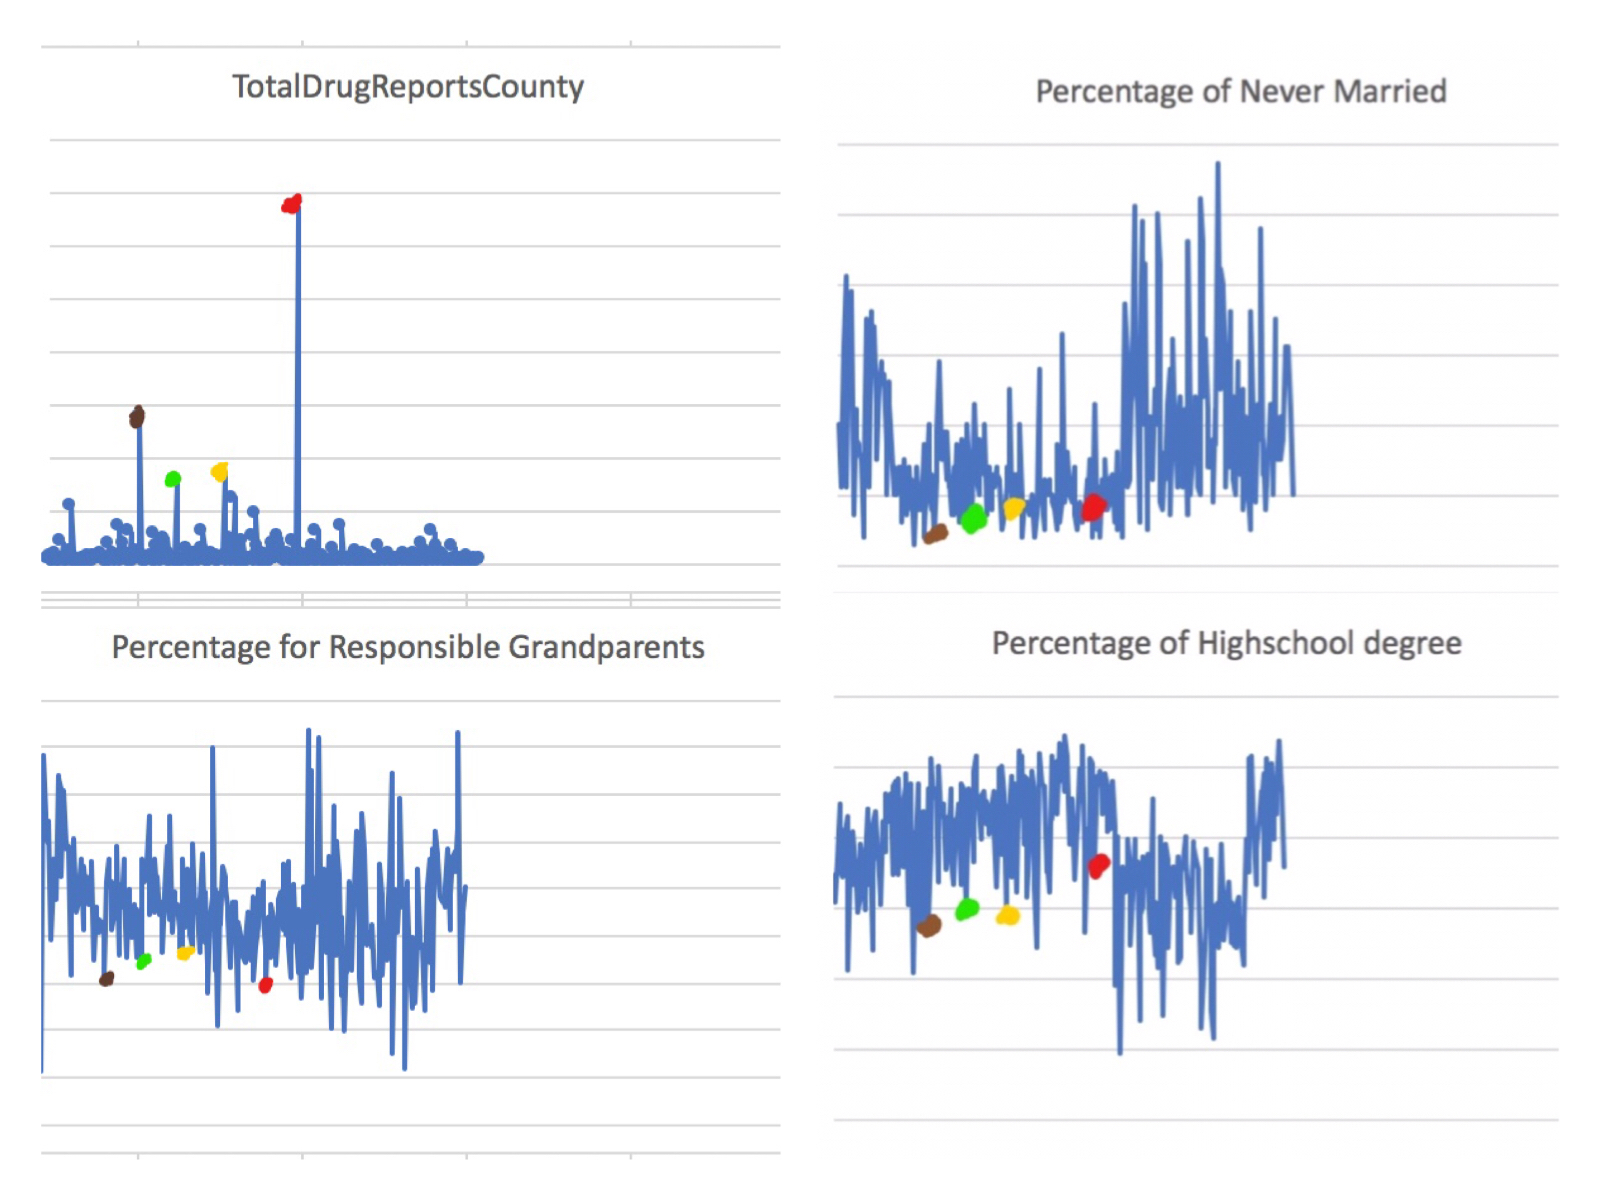
\includegraphics[width = \textwidth, height = 10.5cm]{factor.jpeg}
    \caption{Caption}
    \label{factors}
\end{figure}

From figure \ref{factors} we can tell that, among the three influential factors, the responsibility of grandparents takes a important role in reducing the rate of using drugs. In comparison to the graph of that factor, the other two factors, "never married" and "high school degree" are mild but still shows their importance in the graph.\\

U.S. Census socio-economic data provides a detailed table about different household status such as marital status, fertility, as well as grandparents raising children or not. We examine by plotting the data in each county in accordance with the number of heroine reports in that county to see if the critical points of the selected socio-economic data mostly meets that of the number of heroine reports on the graph. \\



\subsection{Refine the Model }
In the previous section, we find the important factors from the U.S. Census socio-economic data that tightly associate with the current opioid-use level. By implementing these factors into Equation \ref{state}, we gain a more precise function of CA modeling.
\begin{equation}
   D^t_{i,j} = \{S_{i,j}^t,\text{ INF}^t_{i,j}, g, d, m\},
   \label{new}
\end{equation}
~\\
where\\
$g$ is the percentage of people in the county that do not have responsible grandparents, \\
$d$ is the percentage of people in the county that have education level lower than high school, \\
$m$ is the percentage of people in the county that are not married, \\
and in this case we take $g = 5, d = 1.5$ and $m = 1$. \\

\subsection{Possible Actions}
From our model, we found out that the control of $k$ and $l$ is very important. As $k$ and $l$ decreases, the spread of the drug will slow down drastically. Therefore, we have to find effective ways to control the value of $k$ and $l$. Since $k$ and $l$ represents the influence of the neighborhood counties, we think it is important to control the transportation of drugs between areas. One strategy we could use is to post security check on main roads or gas stations on roads to cut off the drug flow and so further decrease the values of $k$ and $l$. 

Other factor that influence the variation of the number of reports is the internal increasing rate $\rho$. This factor represents the growth of drug population results from factors other than the influence of other areas. We can decrease this factor by invest on good drug treatment, as well as take good care of susceptible people who have access to the drug but have not started yet.

By taking these actions, the main reason of the increase of the drug population would be very well-controlled and so the spread could slow down consequently.

%since we notice that with lower percentage of responsible grandparents in a certain county, the total drug report in that county is higher than the mean value of drug report in that state. Similarly, with the lower percentage of people who have at least high school degrees, the drug report in that county is also higher than the mean value of drug reports in that state, and with the lower percentage of bachelors in a county, 
\newpage
\section{Modelling Results and Description}

According to our model running on each of the 5 states, we have predicted the trend and the spread of the drugs within each state.
\subsection{Part 1: Solution Analysis Based on the Inspection of the First Data Set}

Our first model was based on the data provided by the file MCM\_NFLIS\_Data.xlsx. Following is some example of the result yield by our model:
\subsubsection{Spread and Characteristic}
The following is an example of the State of Ohio of the result we had from the model:
\begin{figure}[H]
    \centering
    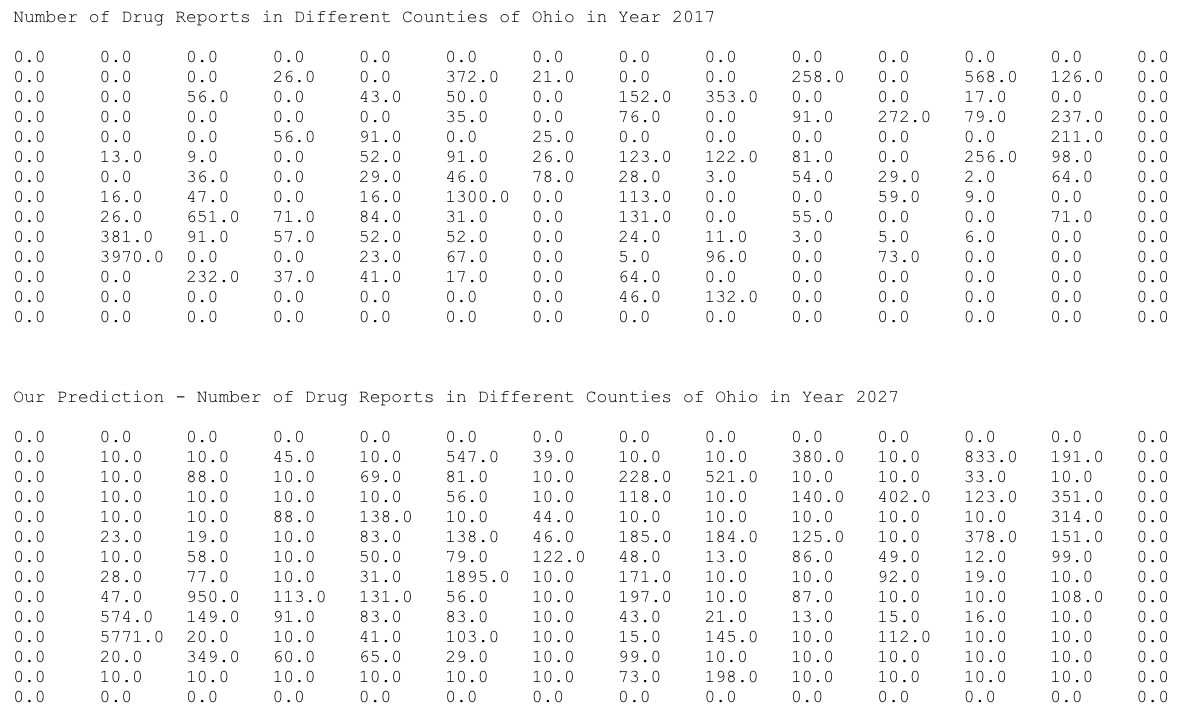
\includegraphics[width = \textwidth]{OHH27.png}
    \caption{Possible Spread of Heroin in Ohio in Year 2027. The 0's on the edges are only for the convenience of the code, there is no actual meaning to them.}
    \label{OHH27}
\end{figure}
Notice that for each state, the development of the local drug community is largely dependent on the larger drug counties, or similarly, more urbanized counties. As the time evolves, the number of drug reports within that sate would increase at a certain rate and it would also influence the counties around it. 

One thing we believe that the US government has to worry about is that there might be appearance of drug users in nearly all of the counties, even if the counties where no drug is reported. In the future, these counties would eventually have more than 20 reports and start to develop its own drug community within itself.

With the threshold level we set at 20, where the drug community would grow intrinsically within the county, our model predicted that roughly after 18 years, all counties might entered the status of rapid growth.

Therefore, we think the most important task for the U.S. government, despite the law enforcement on the drug heavy areas, they should do more on the area that are not originally drug infected instead.

\subsubsection{Possible Starting Region}
By using Equation \ref{backwards}, we can get the possible starting point of each type of drug in each sate. Following are some examples of the result yield by our model. 
\begin{figure}[H]
    \centering
    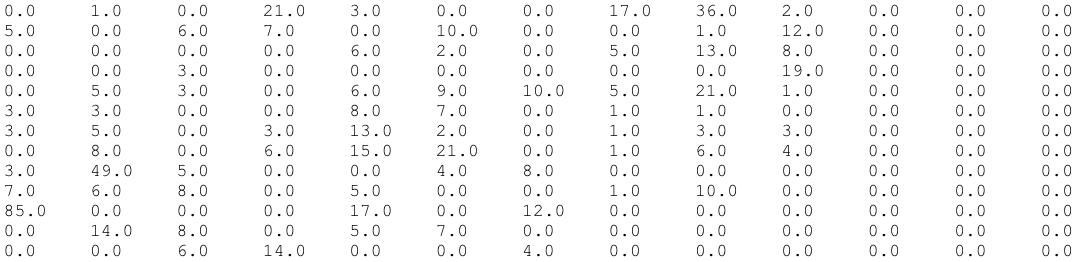
\includegraphics[width = \textwidth]{OHH02.png}
    \caption{Possible Synthetic Opioid Spread in Ohio in Year 2002}
    \label{OHS02}
\end{figure}

\begin{figure}[H]
    \centering
    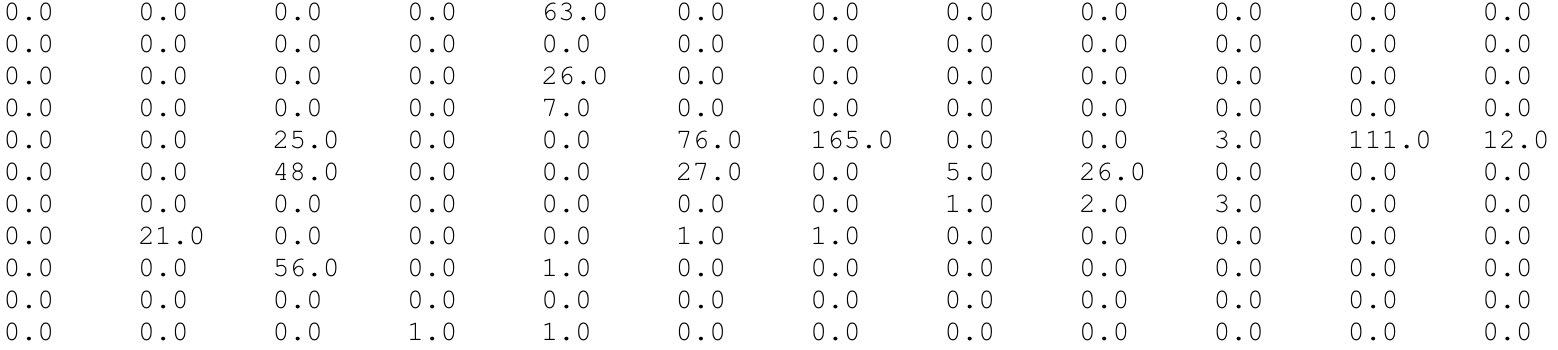
\includegraphics[width = \textwidth]{WVH02.png}
    \caption{Possible Heroin Spread in West Virginia in Year 2002}
    \label{WVH02}
\end{figure}

By looking at those largest points in the resulting matrix, we assume that those points could represent the counties where the drugs initially started. For example in Figure \ref{OHS02} for the Synthetic Opioids in Ohio, the larger numbers are 85, 94 on the bottom left and 36 on the top right. Therefore, we conclude that the Synthetic Opioid spread might first start from those regions where in map represents Hamilton, Montgomery and Cuyahoga. From the second chart, we found that the possible starting point for Heroin in West Virginia could be Kanawha.

By similar reasoning, we get the table below for possible starting points for two different drugs:
\begin{table}[H]
    \centering
    \begin{tabular}{|c||c|c|c|c|c|}
    \hline
       State  & PA & OH & KY & VA & WV \\
       \hline
       Heroin &Philadelphia &Montgomery & Jefferson & Richmond & Kanawha \\
       \hline
       Synthetic Opioid& Philadelphia &Hamilton &Jefferson& Richmond & Pulaski\\
       \hline
    \end{tabular}
    \caption{Possible Starting Points}
    \label{tab:my_label}
\end{table}

\subsubsection{Drawback}
There are some possible flaws of our model since we are doing this without extra data. There are drastic changes in drug uses, especially in 2014, the uses of Heroin and Synthetic Opioid increase in a extremely high rate such that our model is not able to predict this drastic change. 

Also there are some drastic decreases with no obvious reason. For example, the Monongalia county at West Virginia experienced a quick decline on drug usage but we cannot find any pattern underline that unusual change. Thus we assume this might due to sudden law enforcement. However, since this is only a special case, we did not add this feature to our model otherwise it would affect the result of other counties that do not own this characteristic.

\subsection{Part 3: Analysis of Strategy Used}
In order to control the outrageous rate of increment of drug reports and drug taken by people every year, we think it is important to control the use of fentanyl, as well as to protect the counties with no or little drug users. As we mentioned above, with the amount of heroin taken by drug user every year does not change very much, it is important to control the use of synthetic opioids like fentanyl and its related drugs. More importantly, it worth more concern to protect the counties with no or little drug users. As we analyzed the data, we found that many counties that did not have drug report or just had little, but had other counties with higher drug reports surrounded them, would have a rise in the drug report in the next year. Some counties like Harrison, West Virginia, had only 35 reported heroin use in year 2010, but the number rose to 265 in year 2016. Part of the reason for the rapid growth may be that counties above Harrison, Merion and Montogomery, had much higher numbers of heroin uses reported in these years.
\newpage
\section{Strengths and Weaknesses}
\subsection{Strengths}
\begin{itemize}
    \item As we use CA algorithm to calculate the number of drug reports in the past and to predict the contingent number of drug reports in the future, our calculating time spent on the program is negligible, since the algorithm we use is pretty fast, and the result returned is reliable.
    \item 
\end{itemize}

\subsection{Weaknesses}
\begin{itemize}
    \item As we convert the actual map data to Cellular Automaton, we neglect counties with small reports number and relatively very small areas. Since both areas and numbers of reports are fairly small, neglecting them is less likely to cause serious errors on our output.\\
    However, since we fit each county into small grids, each of which has eight neighbors, the distance factor and neighbor information might  deviates the modelling output from the actual data. This chiefly happens when the area of the county is small in comparison to most of its neighbors. 
    
    \item Our model would be better if we are given the population data for each county therefore we can compute percentage of drug users instead of just the pure number. 
\end{itemize}
\newpage
\section{Memo to the Chief Administrator}
Dear Chief Administrator,
~\\

With the provided data of drug reports in the past eight years, we find that the place for the most drug incidents to occur is changing dramatically. In the year 2010, the county that had the most drug reports for the synthetic opioids among the five counties given was Philadelphia, Pennsylvania, with the Hamilton, Ohio and Jefferson, Kentucky were the three counties with the most number of drug reports. Yet starting from year 2013, the state that had the maximum number of synthetic opioids drug reports changed to Montgomery, Cuyahoga and Hamilton, Ohio.
~\\

The case for drug reports of heroin is somewhat different from the case of synthetic opioids: in the year 2010, the top three counties that had the maximum number of drug reports were Philadelphia, Pennsylvania, Allegheny, and Hamilton, Ohio. In the year 2017, the counties that had the most number of drug reports were Philadelphia, Pennsylvania, Cuyahoga, and Hamilton, Ohio. Unlike the statistics that the synthetic opioids report gave, the number of drug reports of heroin in Pennsylvania is much higher than that of synthetic opioids, but both of the reports show that Ohio needs to control the wild spread of synthetic and non-synthetic opioids in itself. In fact, the number of drug reports from Ohio almost doubled in the past eight years, with the starting point of which is also very high.
~\\

More than the above points mentioned, from the year 2015, the number of synthetic opioids used in the five states rose dramatically: in the year 2014, the largest number of drug reports was 388, while in next year, the largest number became 1592, and in year 2017, the largest number became 5425. During our analysis of the data, we found out that the sudden growth of synthetic opioids was because the birth of fentanyl and its related drugs. In year 2010, according to the data provided, there was no report of use of fentanyl, but in year 2015, when the number of synthetic opioids grew suddenly, fentanyl appeared, and the amount of fentanyl being used in the following years was increasing annually. 
~\\

In order to control the outrageous rate of increment of drug reports and drug taken by people every year, we think it is important to control the use of fentanyl, as well as to protect the counties with no or little drug users. As we mentioned above, with the amount of heroin taken by drug taker every year does not change much every year, it is important to control the use of synthetic opioids like fentanyl and its related drugs. More importantly, it worth more concern to protect the counties with no or little drug users. As we analyzed the data, we found that many counties that did not have drug report or just had little, but had other counties with higher drug reports surrounded them, would have a rise in the drug report in the next year. Some counties like Harrison, West Virginia, had only 35 reported heroin use in year 2010, but the number rose to 265 in year 2016. Part of the reason for the rapid growth may be that counties above Harrison, Merion and Montogomery, had much higher numbers of heroin uses reported in these years. \\

Therefore, in order to control the annual growth of drug use in the United States, it is urgent to control the use of fentanyl, and to limit or prohibit the drug circulation among states with high number of drug reports every year and states with seldom drug reports every year. After solving these two major concerns, we believe that the life in the United States may be much better. \\

Thank you for taking your time reading our suggestions. We sincerely hope that this memo will offer some useful ideas and advice.

% - - - - - - - - - - - END Model Design - - - - - - - - - - -



% - - - - - - - - - - - Model Solution - - - - - - - - -

% labels allow you to cross-reference a section later in the document, without having to remember its number
%  - - - - - - - - - - - - - - - - - - - - - - - - - - - - - -
% Delete existing text when writing your own report.


 

% - - - - - - - - - - - END Discussion - - - - - - - - - - -



% - - - - - - - - - - - References - - - - - - - - -
% [1] http://www.comap-math.com/mcm/2019\_MCM-ICM\_Problems.zip


% - - - - - - - - - - - END References - - - - - - - - - - -




% = = = = = = = = = = = = = = = = = = = = = = = = = = = = = = 
%				END YOUR DOCUMENT - did you proofread?
% = = = = = = = = = = = = = = = = = = = = = = = = = = = = = = 
\end{document} % End of document. Nothing after this line will appear in .pdf
% = = = = = = = = = = = = = = = = = = = = = = = = = = = = = = 